\documentclass[12pt, a4paper]{memoir}
\usepackage{amsmath}
\usepackage{graphicx}
\usepackage{wrapfig}
\usepackage{natbib}

\usepackage[utf8]{inputenc}
\usepackage[english]{babel}
\usepackage{lmodern}
\usepackage[T1]{fontenc}
\usepackage[babel=true]{microtype}

\begin{document}

\frontmatter

\title{M2 Thesis Draft -- Sketch Based Animation of Dancing Couples}

\author{
Sarah Kushner \\
\'Ecole nationale sup\'erieure d'informatique \\
et de math\'ematiques appliqu\'ees, \\
Institut polytechnique de Grenoble, \\
Advisers: Marie-Paule Cani and R\'emi Ronfard\\

\texttt{sarah-anne.kushner@ensimag.fr}
}

\date{\today}

\begin{titlingpage}
\maketitle
\end{titlingpage}


\renewcommand{\abstracttextfont}{\normalfont}
\abstractintoc
\begin{abstract} 
Your abstract goes here... 
\end{abstract}
\abstractintoc

\mainmatter
\section{Introduction}
\subsection{Problem Statement}
3D animation can be a painstakingly tedious activity. To create a desired animation, animators go through the long process of keyframing. Keyframes are set positions that define the start and end points of a movement, sequences of poses which are transformed in time. Typically, animators assign poses to certain frames over time, so that in-between motions can be generated by a computer. To get an accurate animation, artists usually must assign many keyframes, then spend time adjusting and editing them to be more precise. The fact that industry professionals take so much time and effort to do this shows that for an amateur or untrained artist, creating \textit{good} 3D animation is close to impossible.

\begin{wrapfigure}{R}{0.6\textwidth}
\centering
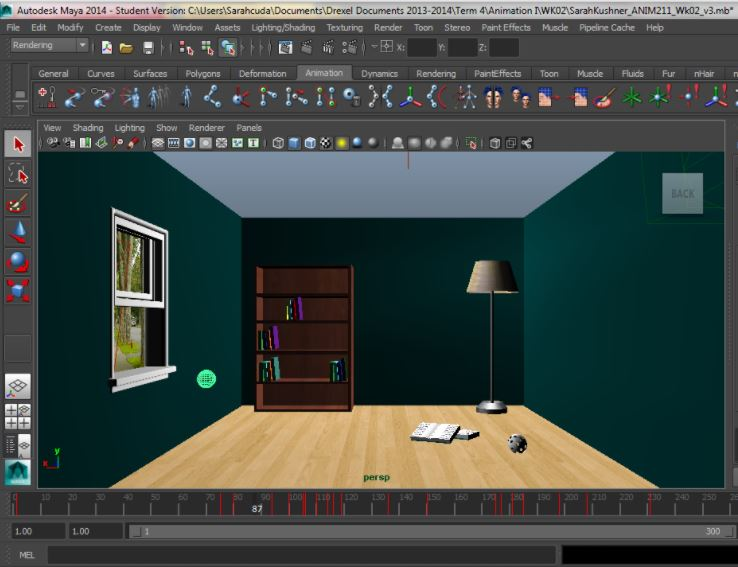
\includegraphics[scale=0.4]{img/keyframe}
\caption{Keyframing.}
\end{wrapfigure}

Researchers in the IMAGINE group at INRIA have noticed this problem. They have made significant progress on a project where they aim to offer more intuitive tools to author 3D digital content. The IMAGINE team has invented (1) a type of notation made especially for posing and animating 3D characters (2) a technique for posing called the line of action, in which a user can draw a line in the shape they want a kinematic chain to take and (3) a technique for animation called space-time sketching, in which a user can draw a line in the path they want a model to take and it will be animated accordingly. As the character follows the path, its model bends and changes shape in a physically realistic way. Their system currently supports creating different movements with the path such as bouncing, rolling, and twisting.

Among the most complicated characters to animate in 3D animation are humanoid characters. To ease this task, animators create a skeleton for their character called a rig, that consists of joints connected by bones to give a structure to the character. Humanoid rigs can range in complexity from (relatively) simple to extremely complicated depending on the amount of detail desired by the user. The structure is a hierarchy of joints that can also be seen as a tree with a root, which in the humanoid case, is usually the pelvis.

\begin{figure}[h!]
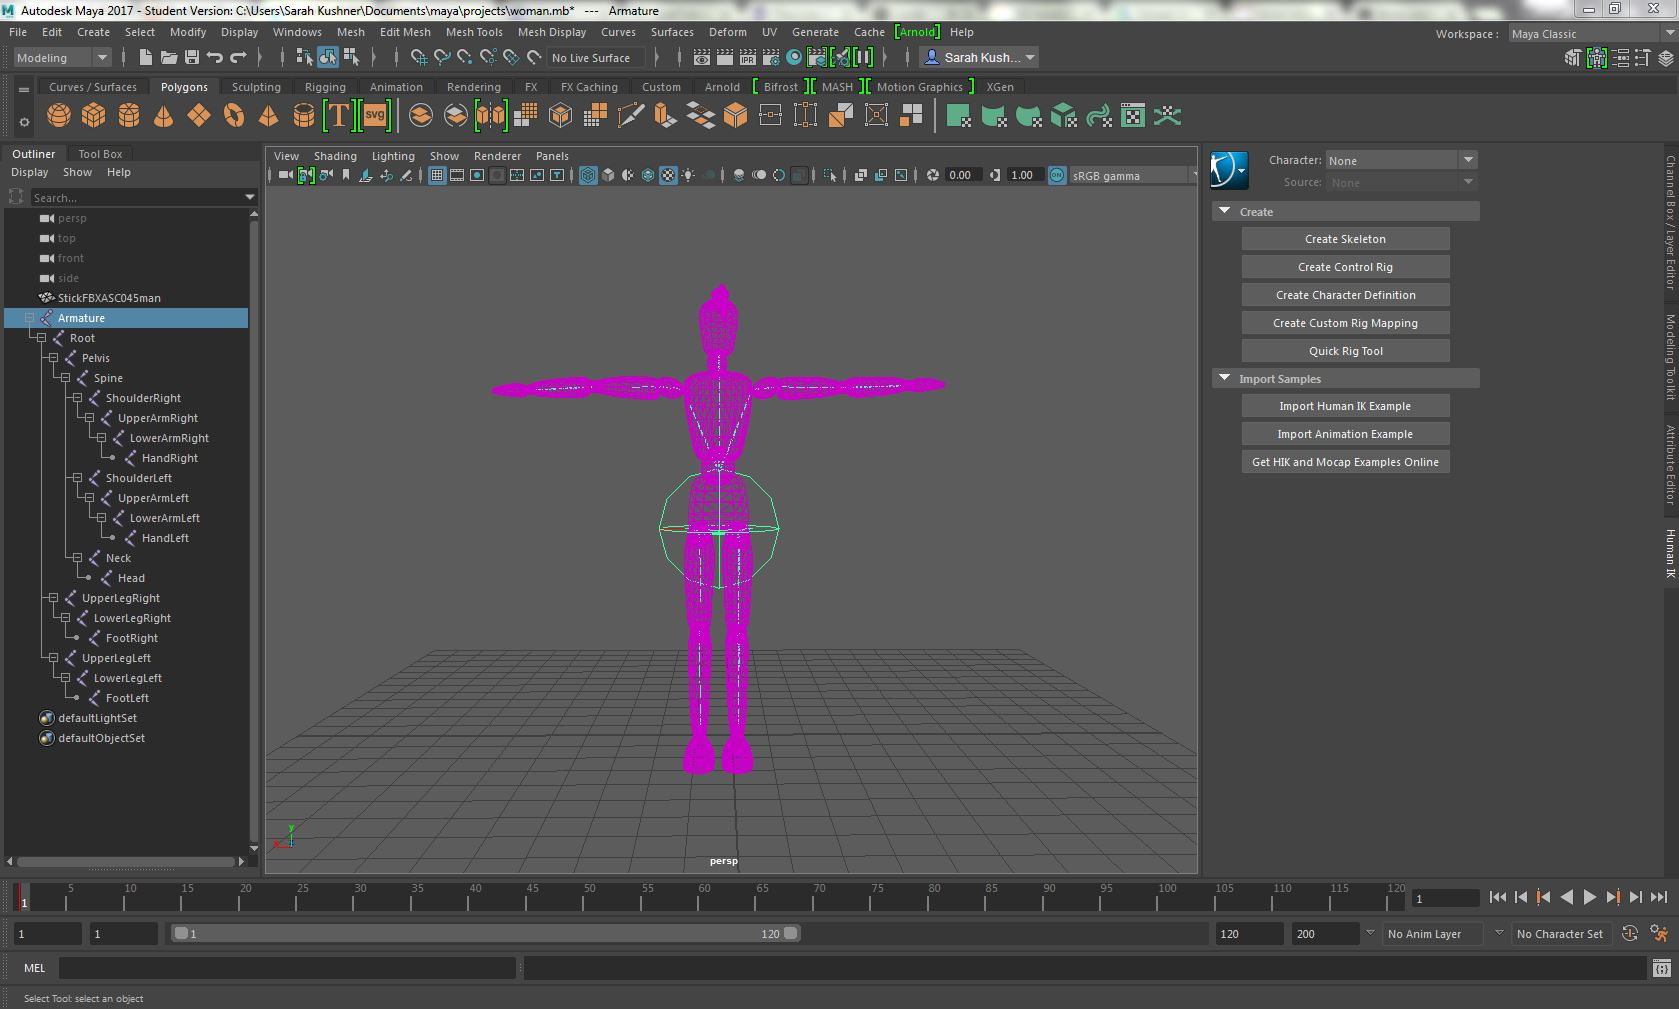
\includegraphics[scale=0.3]{img/skeleton}
\caption{Example of a humanoid skeleton.}
\end{figure}

\subsection{Forward and Inverse Kinematics}
In order to animate this structure successfully, controls are added that allow for forward and inverse kinematics. These controls help the animator move the character into poses that will then act as keyframes.

Forward kinematics is a method of calculating the position and orientation of the end of a kinematic chain (i.e. a hand or foot) given the positions and angles of the joints higher up in the chain all the way to the root. 

Inverse kinematics is the opposite method of forward kinematics. That is, the goal is to calculate the angles and positions of joints in the chain, given the angle and position of just the end of the chain. This goal much harder to reach, seeing that more information needs to be calculated than is given.

\subsection{Multiple Characters}
The animation of multiple characters, along with all the previously mentioned challenges, comes with its own unique set as well. The line of action technique works extremely well for a single humanoid character, and even multiple humanoid characters separate from each other. The problem is discovered when the humanoid characters interact, when they are in close proximity to each other or when they touch each other.


Occlusion?

Collisions

\begin{figure}
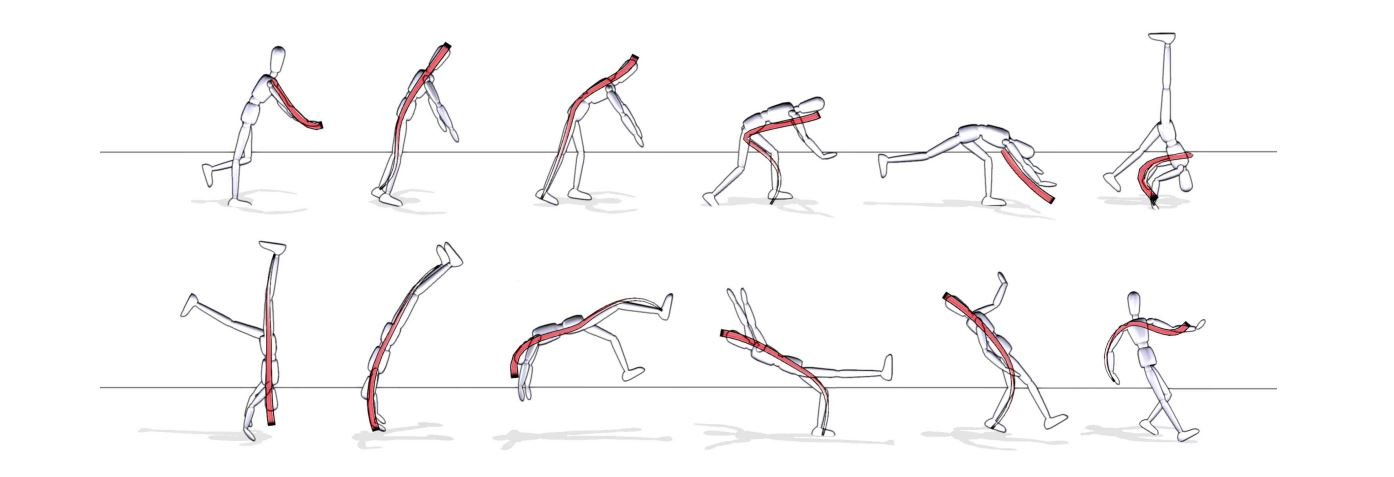
\includegraphics[scale=0.4]{img/baseline}
\caption{One character's keyframes using the line of action technique.}
\end{figure}

\section{State of the Art}
\subsection{sketching for posing and animation}
The Line of Action: an Intuitive Interface for Expressive Character Posing -- 2013\\
Adding dynamics to sketch-based character animations -- 2015\\
Space-time sketching of character animation -- 2015\\
\\
Artist-oriented 3D character posing from 2D strokes -- 2016\\
people in Switzerland also did the posing \\
Sketch to pose in Pixar's presto animation system -- 2015

\subsection{cleaning/editing animation}
FootSee: an Interactive Animation System\\
Footskate Cleanup for Motion Capture Editing\\
SketchiMo: Sketch-based Motion Editing for Articulated Characters -- 2016\\
sketching for editing trajectories and poses

\subsection{retargeting motion}
Retargetting Motion to New Characters\\
Using an Intermediate Skeleton and Inverse Kinematics for Motion Retargeting

\subsection{generating animation}
Motion Graphs\\
Style-Based Inverse Kinematics -- 2004\\
generative models for motion capture sequences used to build animations\\\\
Displacement constraints for interactive modeling and animation of articulated structures -- 1994\\
fitting geometric constraints using physics\\\\
A constrained inverse kinematics technique for real-time motion capture animation -- 1999\\
Dancing-to-Music Character Animation

\subsection{synthesis}
Synthesizing Dance Performance Using Musical and Motion Features -- 2006\\
between music and an animation generated from a motion graph built from motion capture

\subsection{analyzing/classification}
Analysis of impression of robot bodily expression\\
Convolutional Pose Machines

\subsection{graph theory}
FINDING ALL THE ELEMENTARY CIRCUITS OF A DIRECTED GRAPH\\
A New Search Algorithm for Finding the Simple Cycles of a Finite Directed Graph\\
An Algorithm for Combining Graphs Based on Shared Knowledge

\subsection{math/algorithms}
The Conjugate Residual Method for Constrained Minimization Problems -- 2015\\
Constrained Closed Loop Inverse Kinematics -- 2010

\subsection{dance notation}
Sutton Dance Writing\\
Labanotation\\
Benesh Movement Notation


\section{Proposed Solution}
\subsection{Line of Action Notation}
Taking inspiration from Sutton Notation, we propose a new notation for representing the poses of two characters both together and separately.

\begin{figure}[!h]
\centering
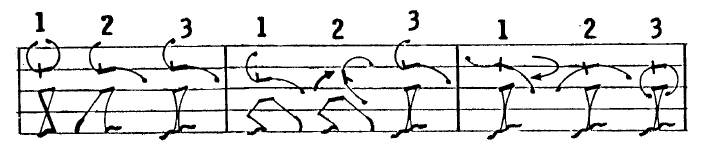
\includegraphics[scale=0.4]{img/sutton}
\caption{An example of Valerie Sutton's Dancewriting.}
\end{figure}

\subsubsection{Common Multi-character Poses}
\begin{wrapfigure}{L}{0.55\textwidth}
\centering
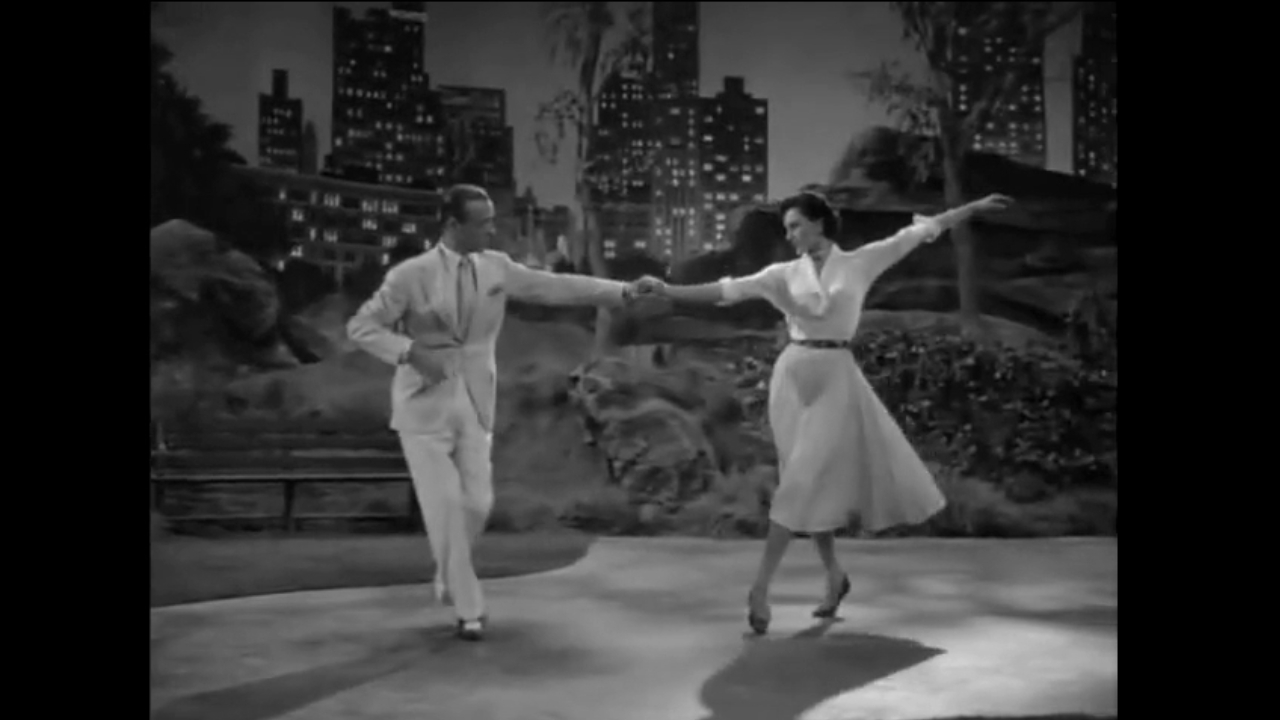
\includegraphics[scale=0.1]{img/bandwagon}
\caption{Dancing in the Dark.}
\end{wrapfigure}

There is a dance scene in the film ``The Band Wagon,'' where Cyd Charisse and Fred Astaire start out by walking together side by side, exchanging twirls until it morphs completely into a swing style dance. This scene is our use case for inventing a notation which extends seamlessly to more than one character.


\newpage
To determine which poses for these dancers were common, I annotated the video with what I thought good keyframes would be if the two characters were treated as one. 

\begin{table}[!htb]
  \centering
  \begin{tabular}{ | c | c || c | c | c | }
    \hline
     & Separate & \multicolumn{3}{c |}{Together}\\ \hline
    1 LOA 
    & &
    \begin{minipage}{.15\textwidth}
      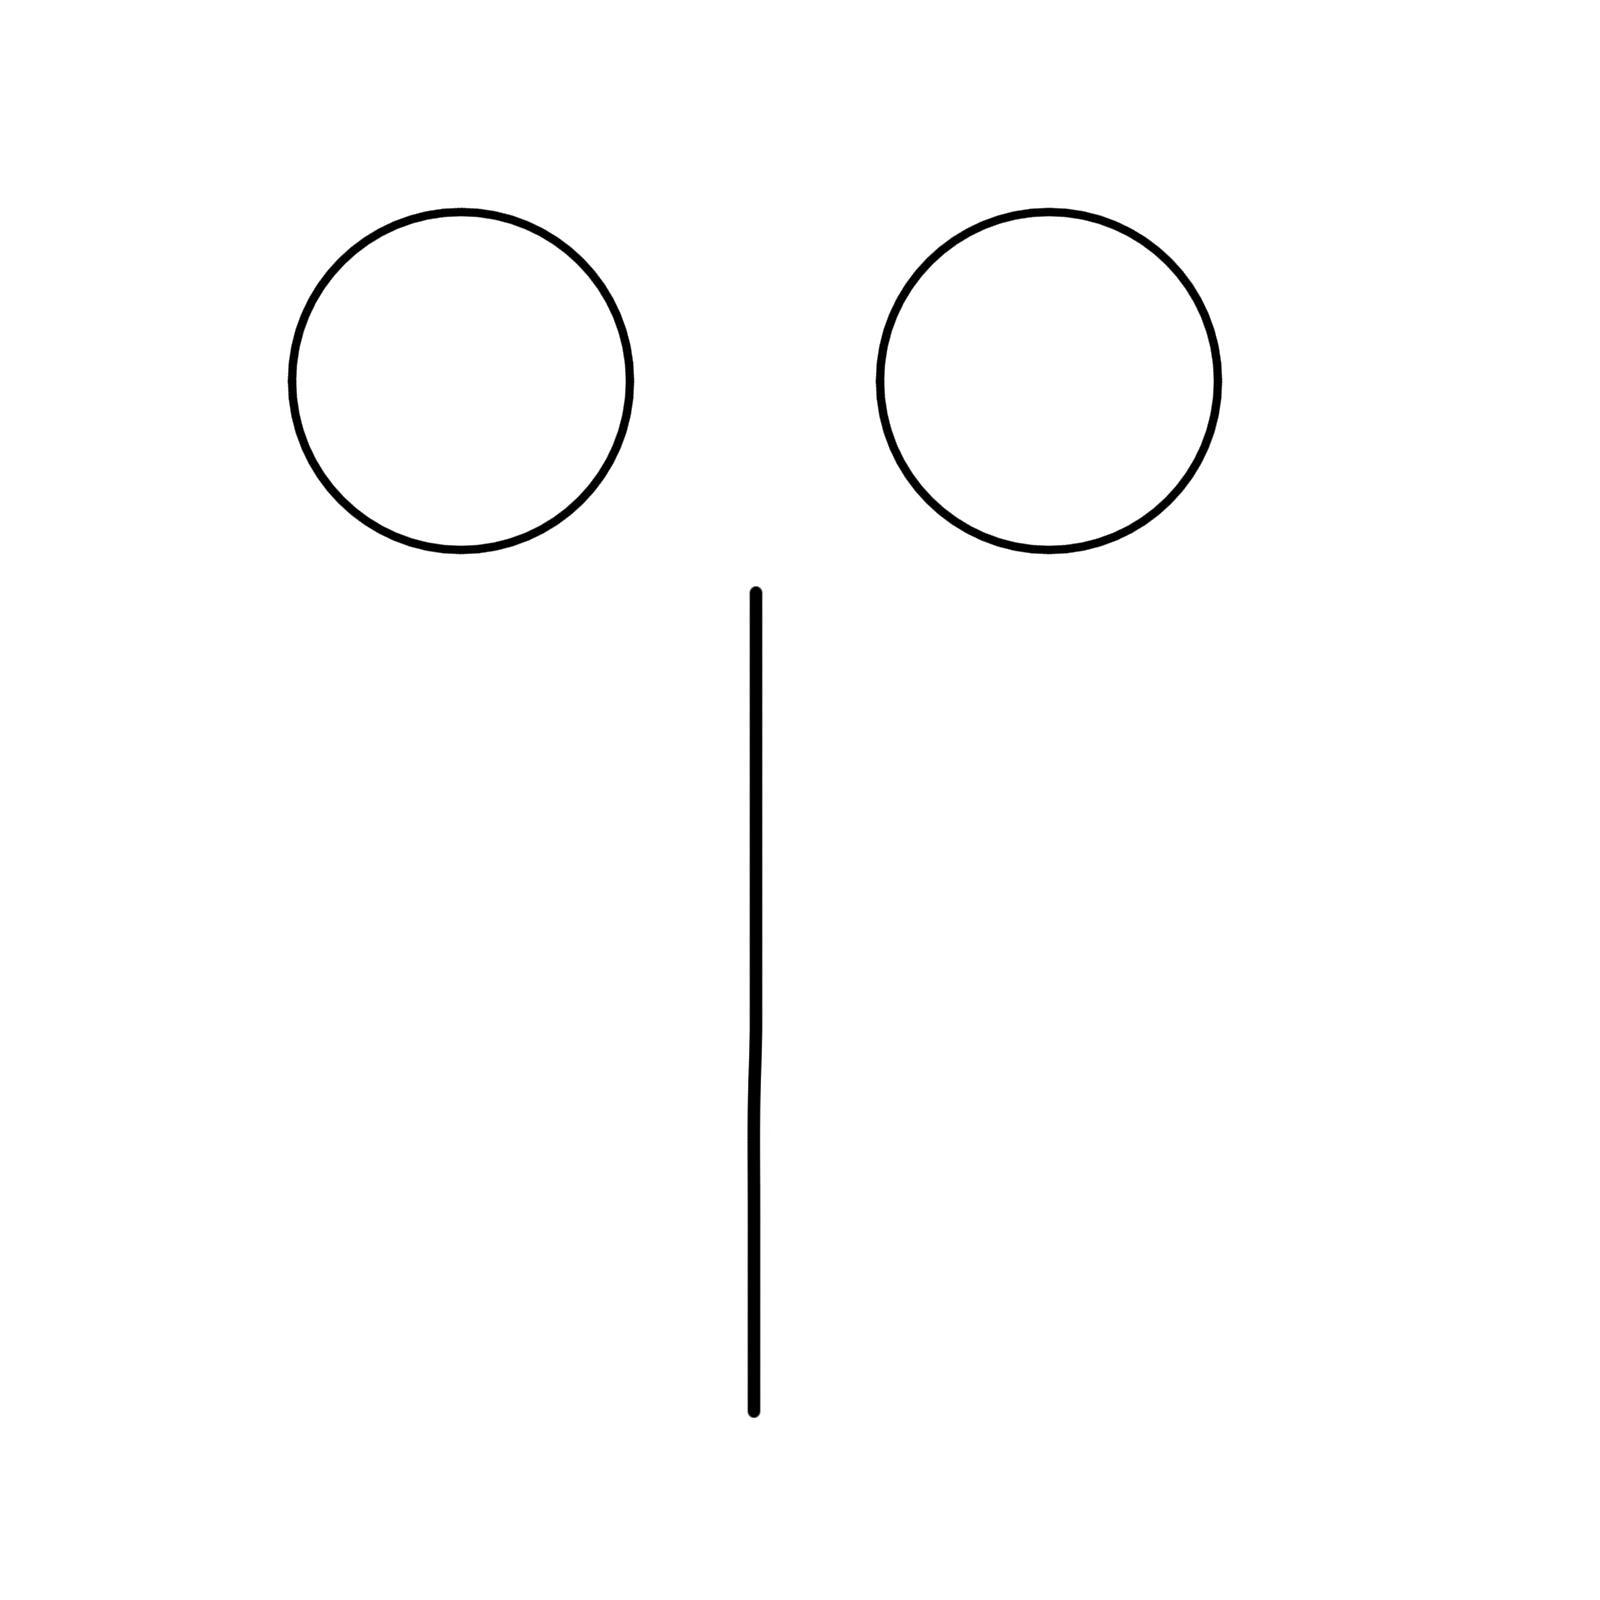
\includegraphics[width=\linewidth, height=20mm]{img/01keyframe}
    \end{minipage} & & \\ 
    \hline
    2 LOA 
    &
    \begin{minipage}{.15\textwidth}
      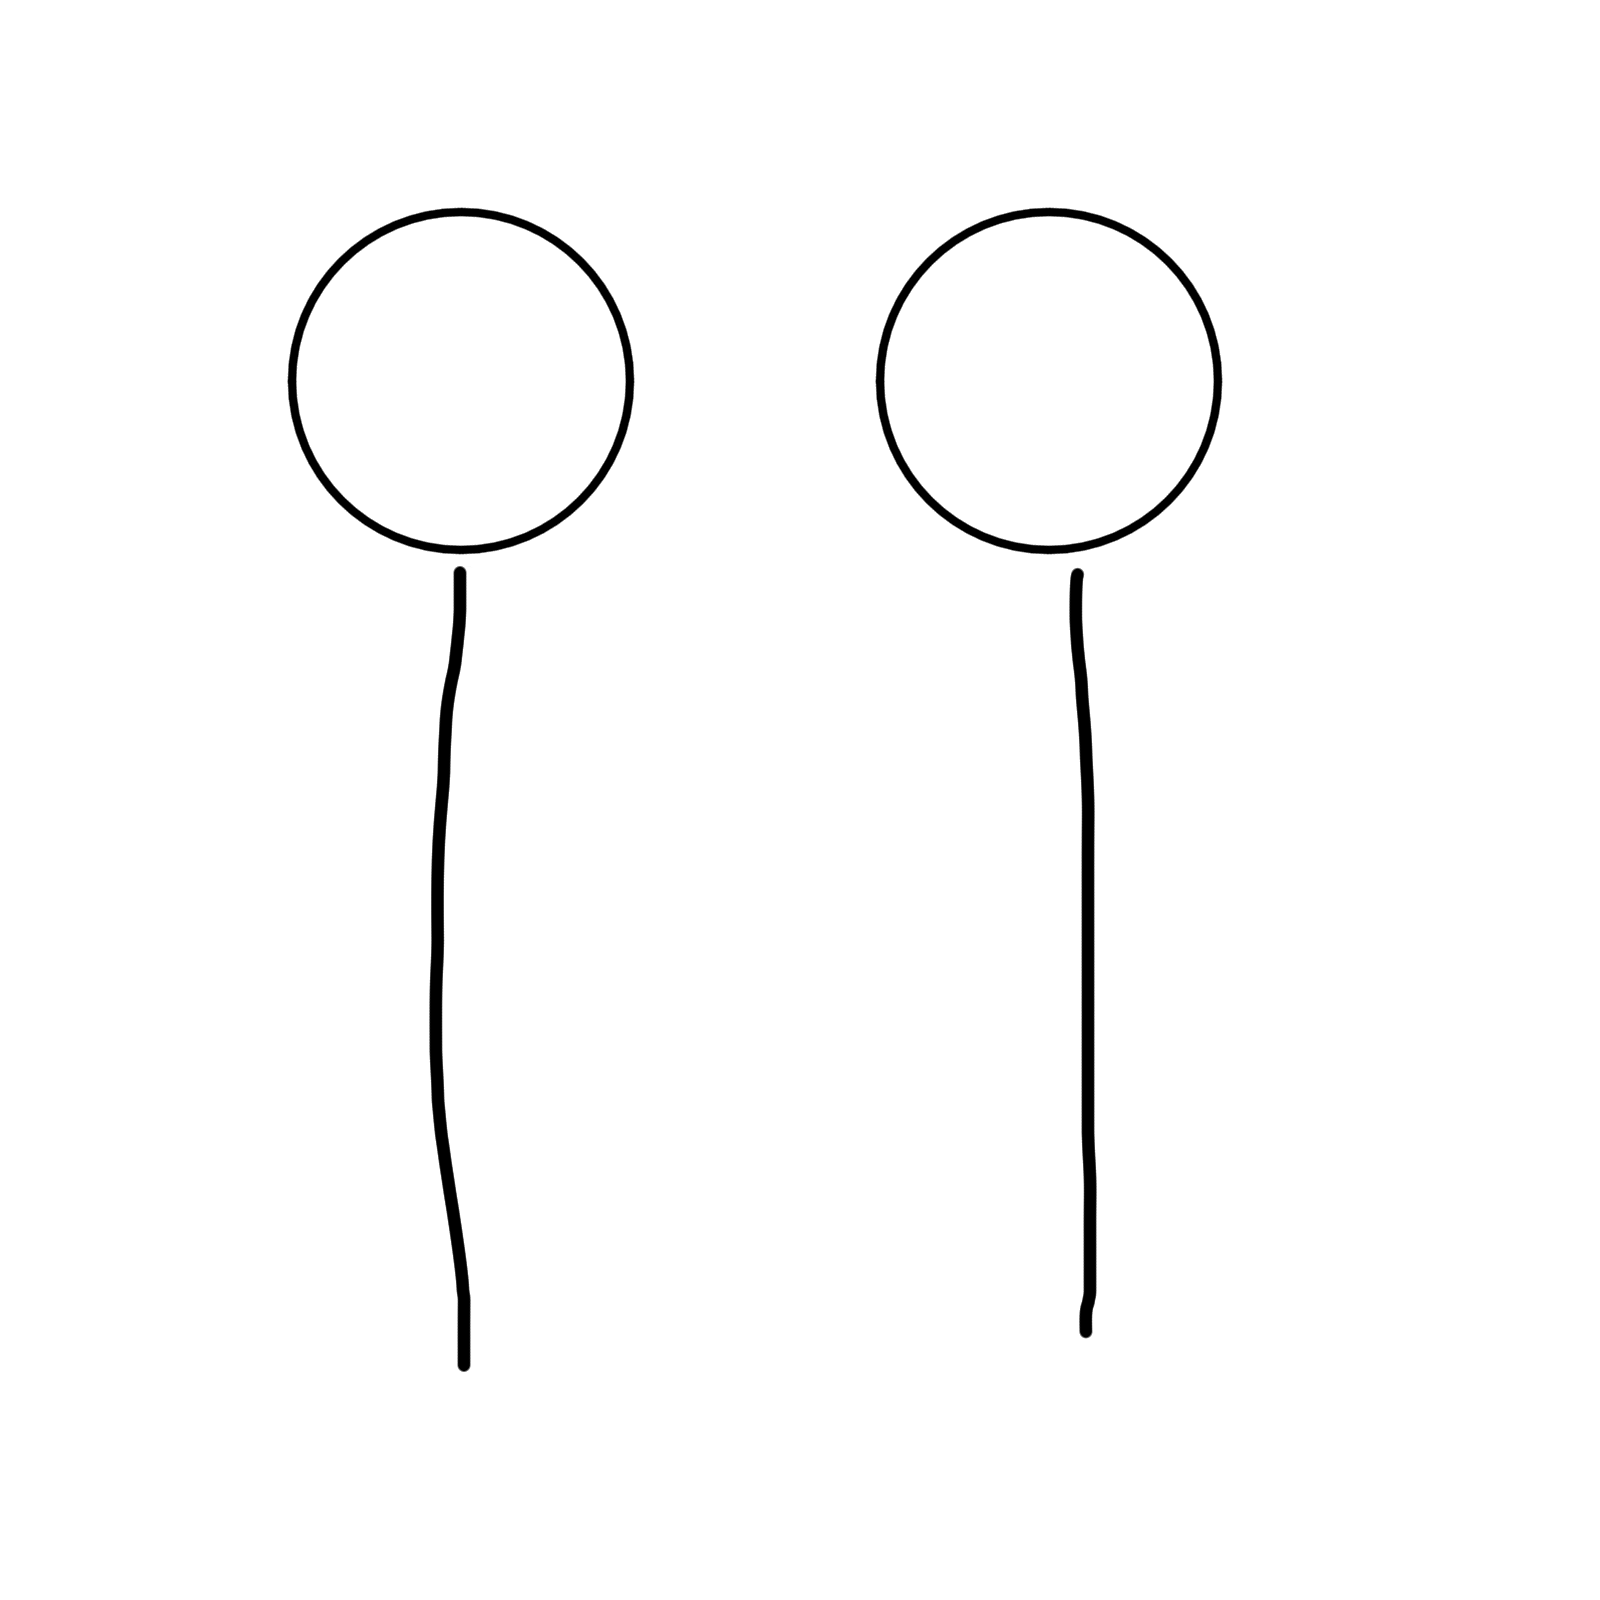
\includegraphics[width=\linewidth, height=20mm]{img/2loa_separate_keyframe}
    \end{minipage}
    &
    \begin{minipage}{.15\textwidth}
      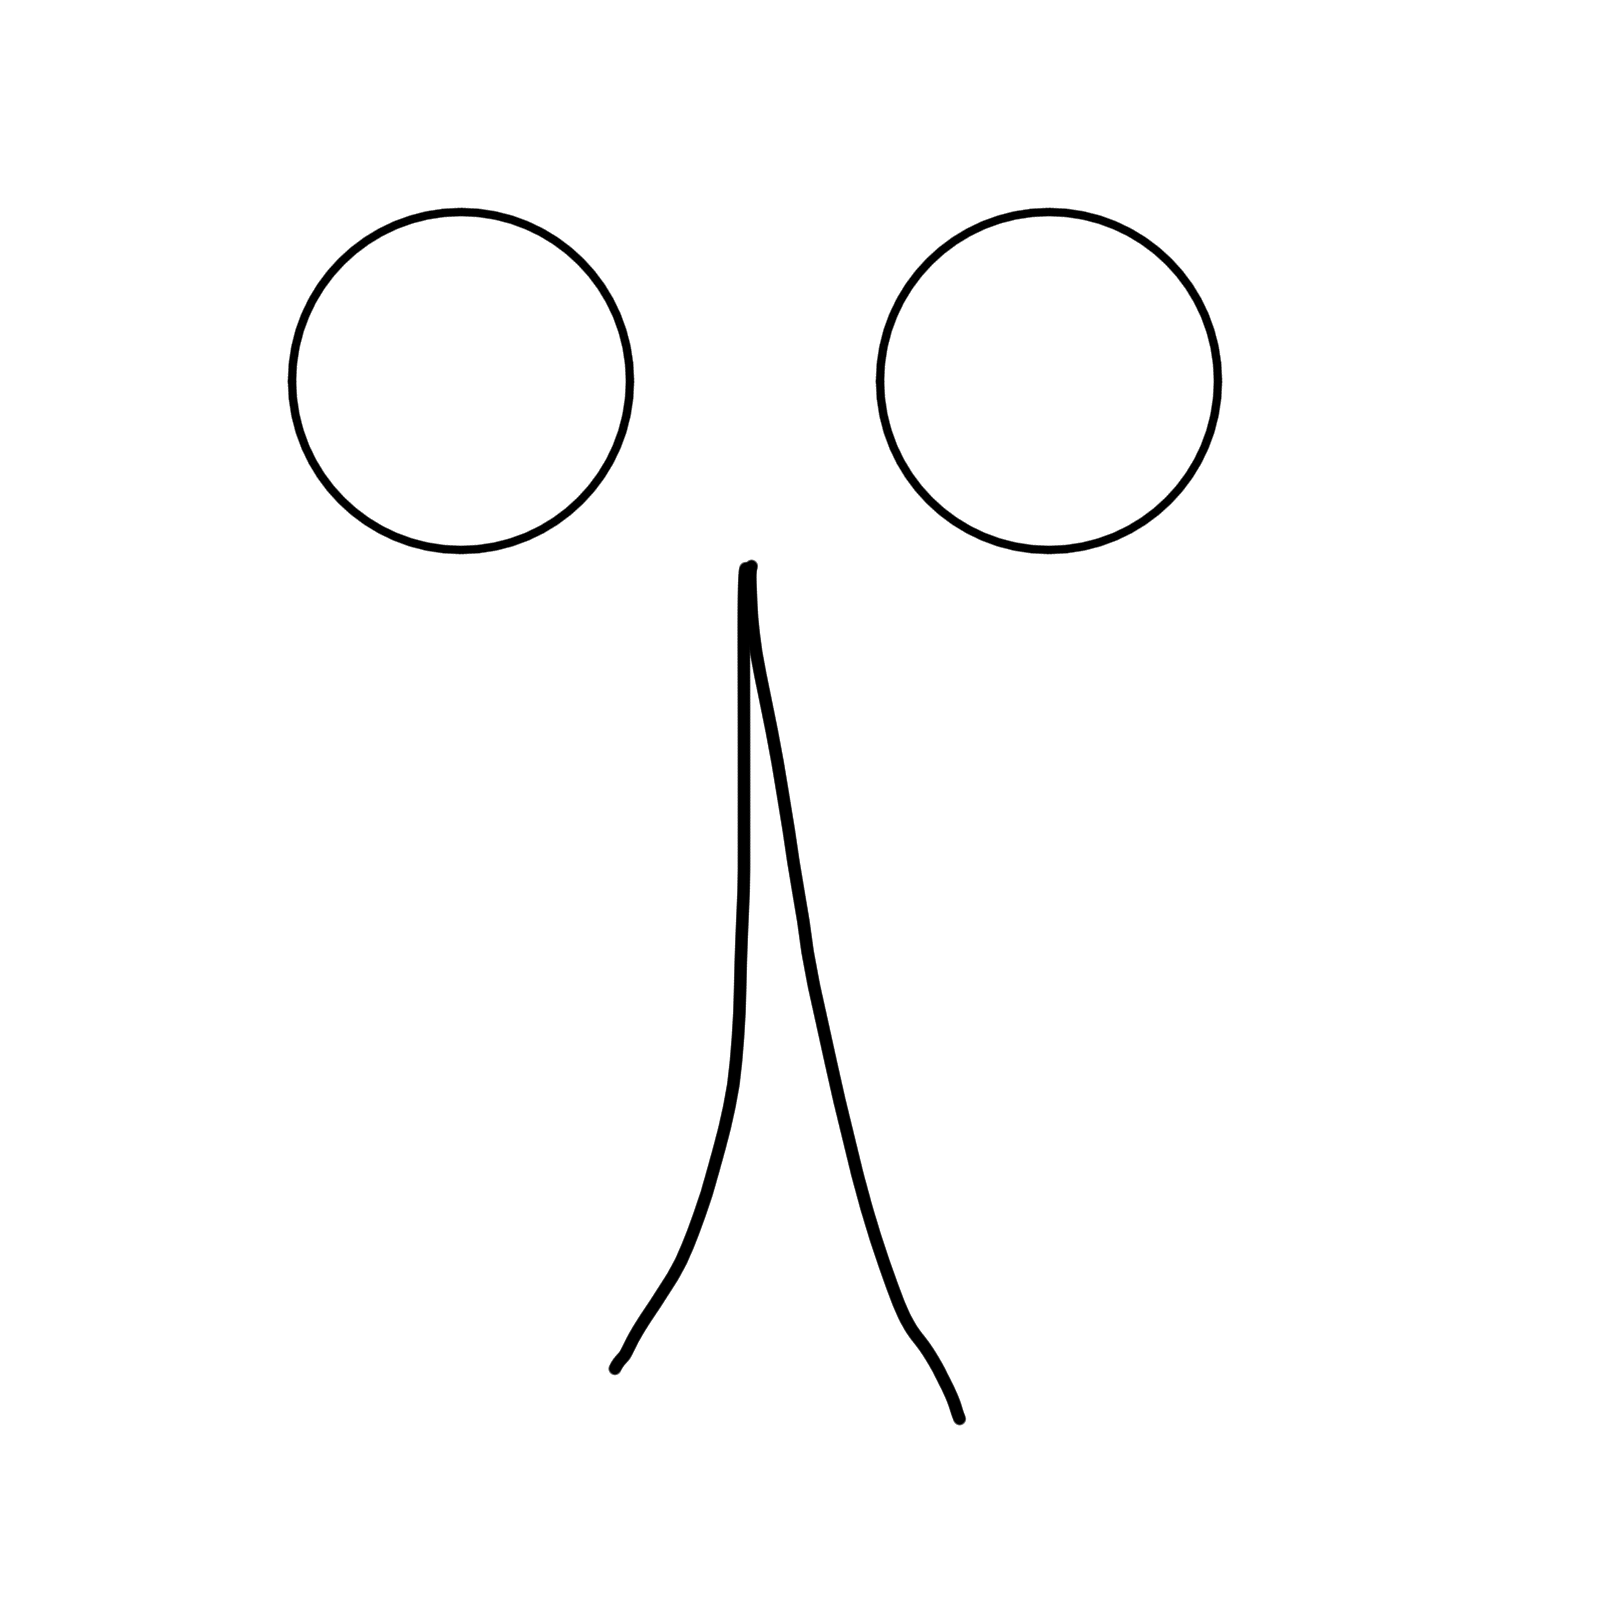
\includegraphics[width=\linewidth, height=20mm]{img/02keyframe}
    \end{minipage}
    &
    \begin{minipage}{.15\textwidth}
      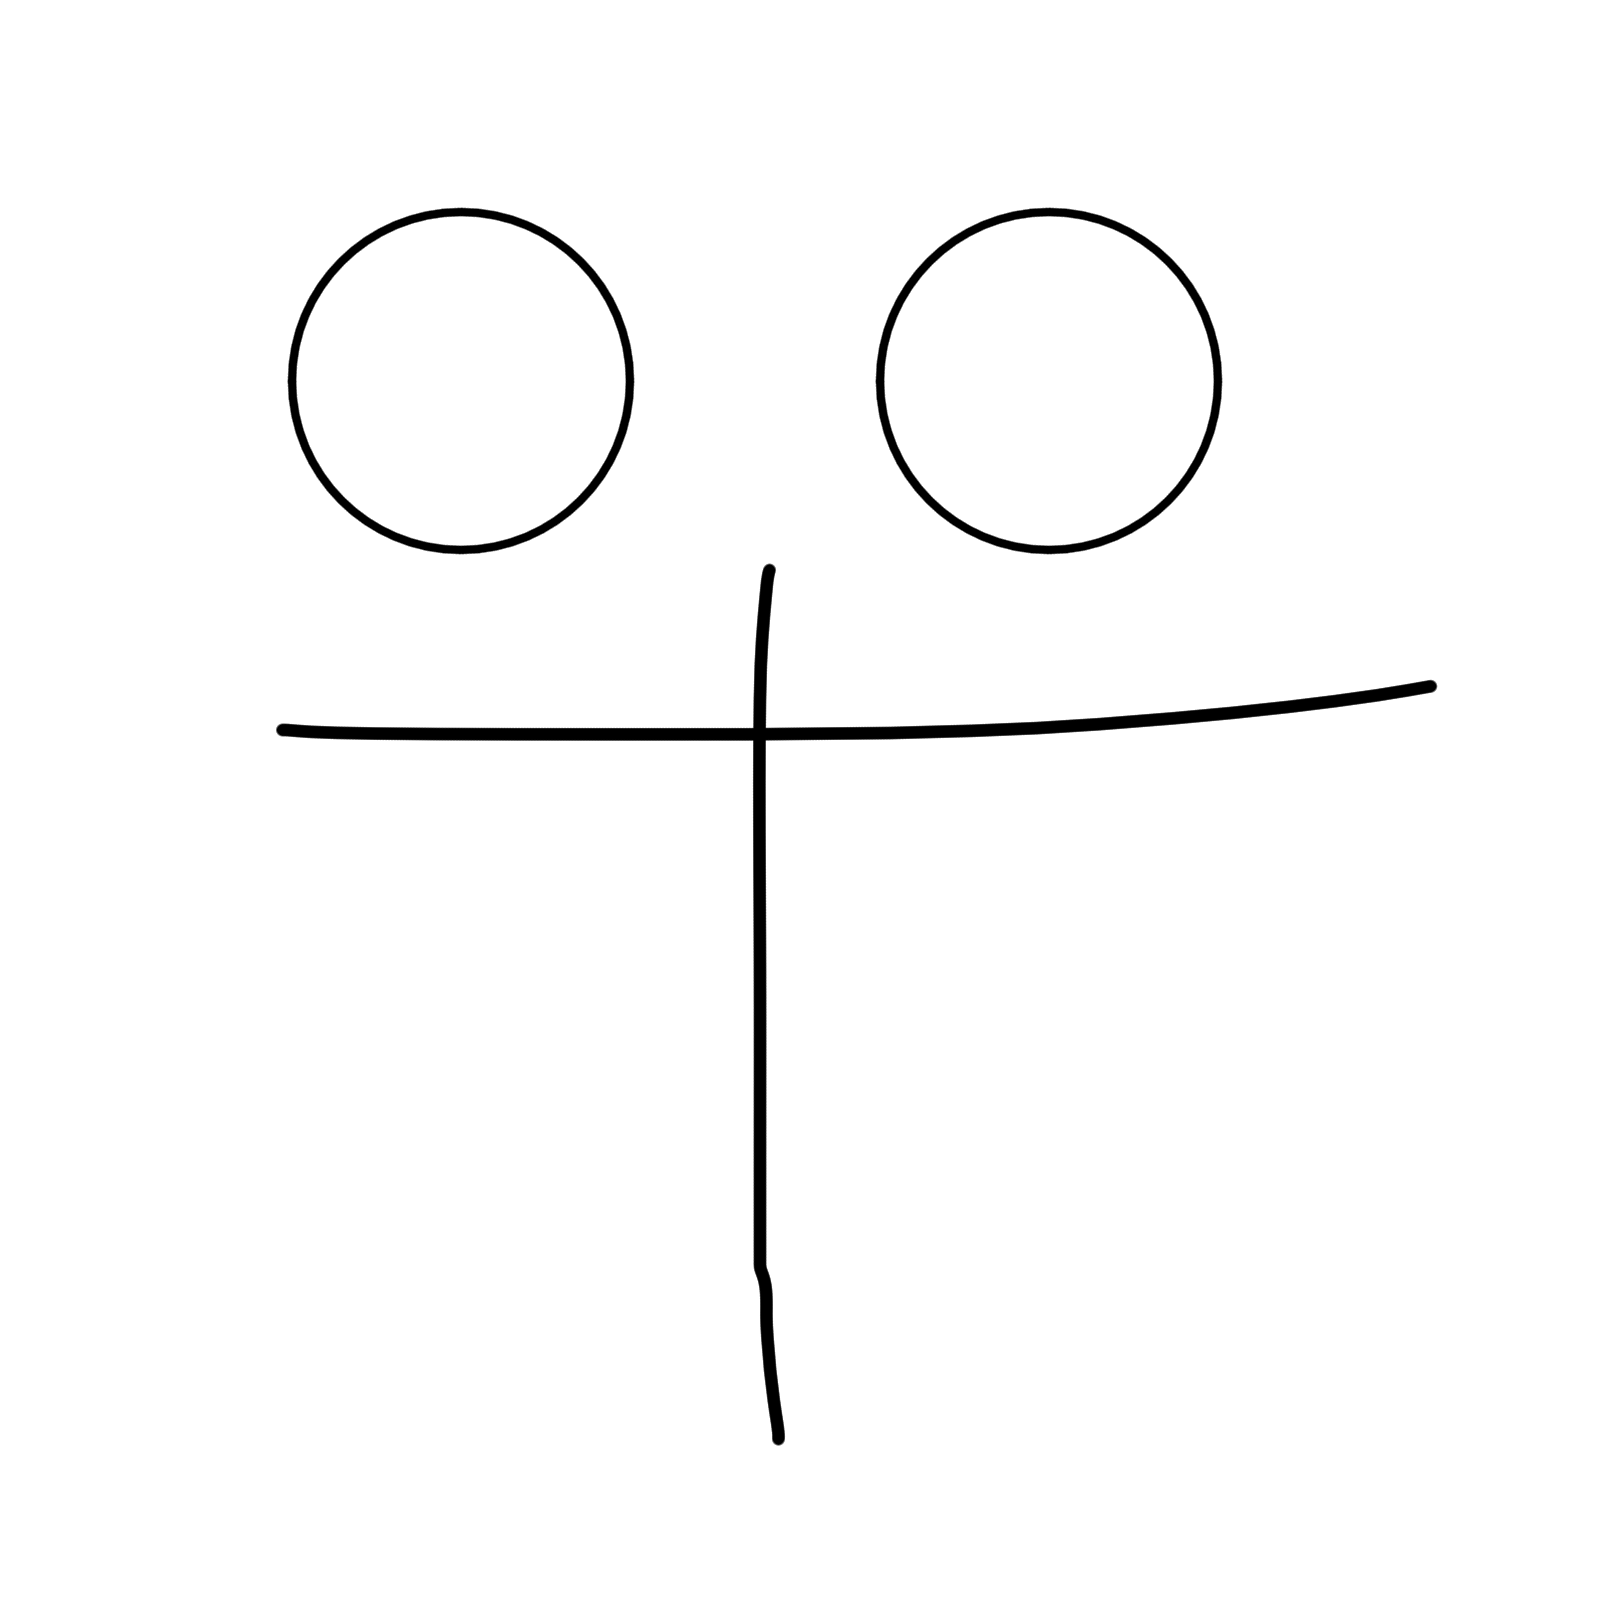
\includegraphics[width=\linewidth, height=20mm]{img/03keyframe}
    \end{minipage} & 
    \\ \hline
    3 LOA 
    &
    \begin{minipage}{.15\textwidth}
      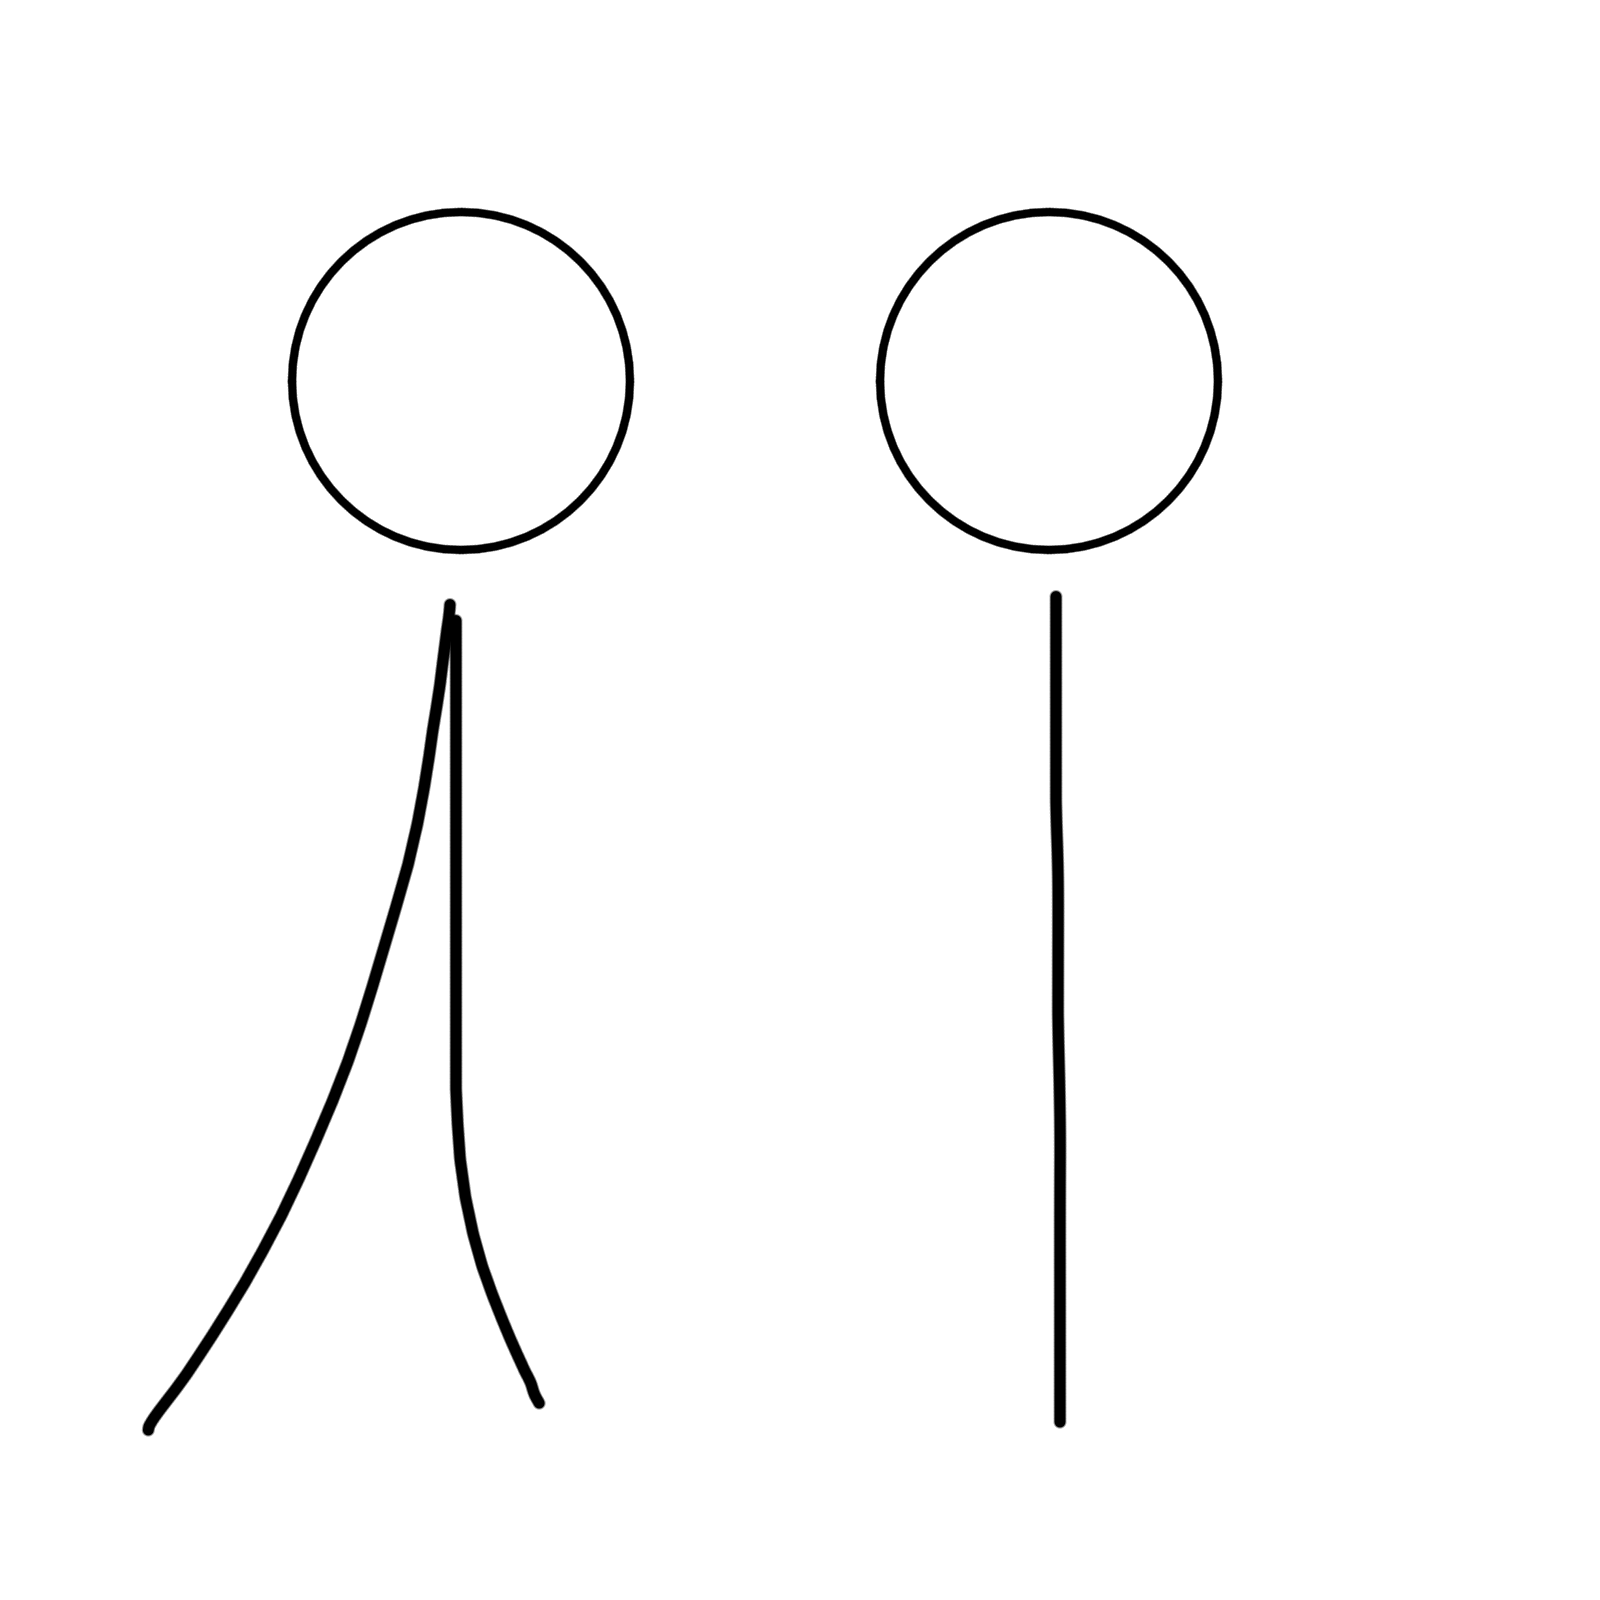
\includegraphics[width=\linewidth, height=20mm]{img/3loa_separate_keyframe}
    \end{minipage}
    &
    \begin{minipage}{.15\textwidth}
      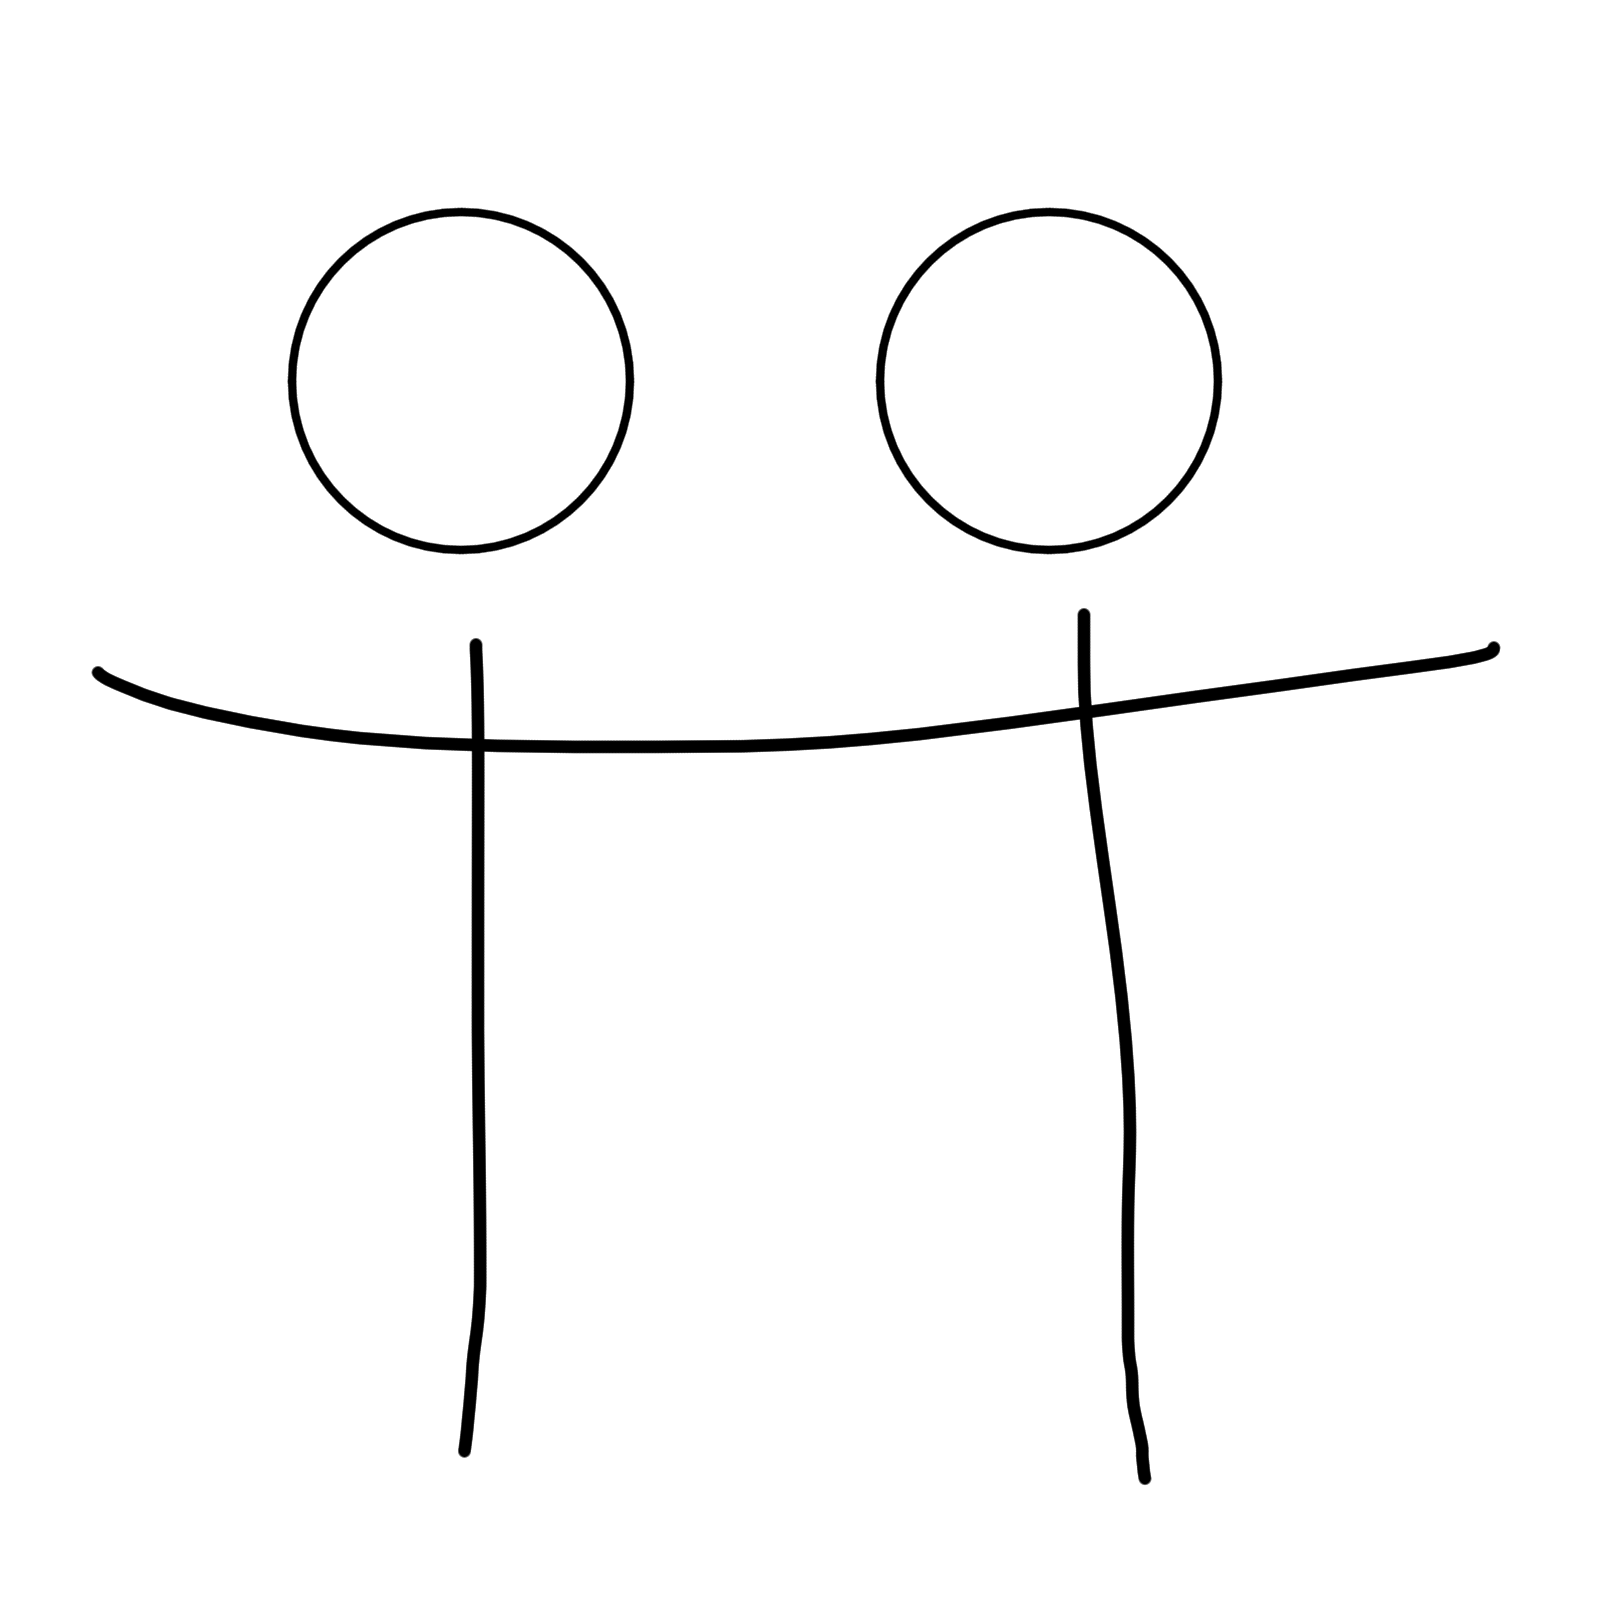
\includegraphics[width=\linewidth, height=20mm]{img/04keyframe}
    \end{minipage}
    &
    \begin{minipage}{.15\textwidth}
      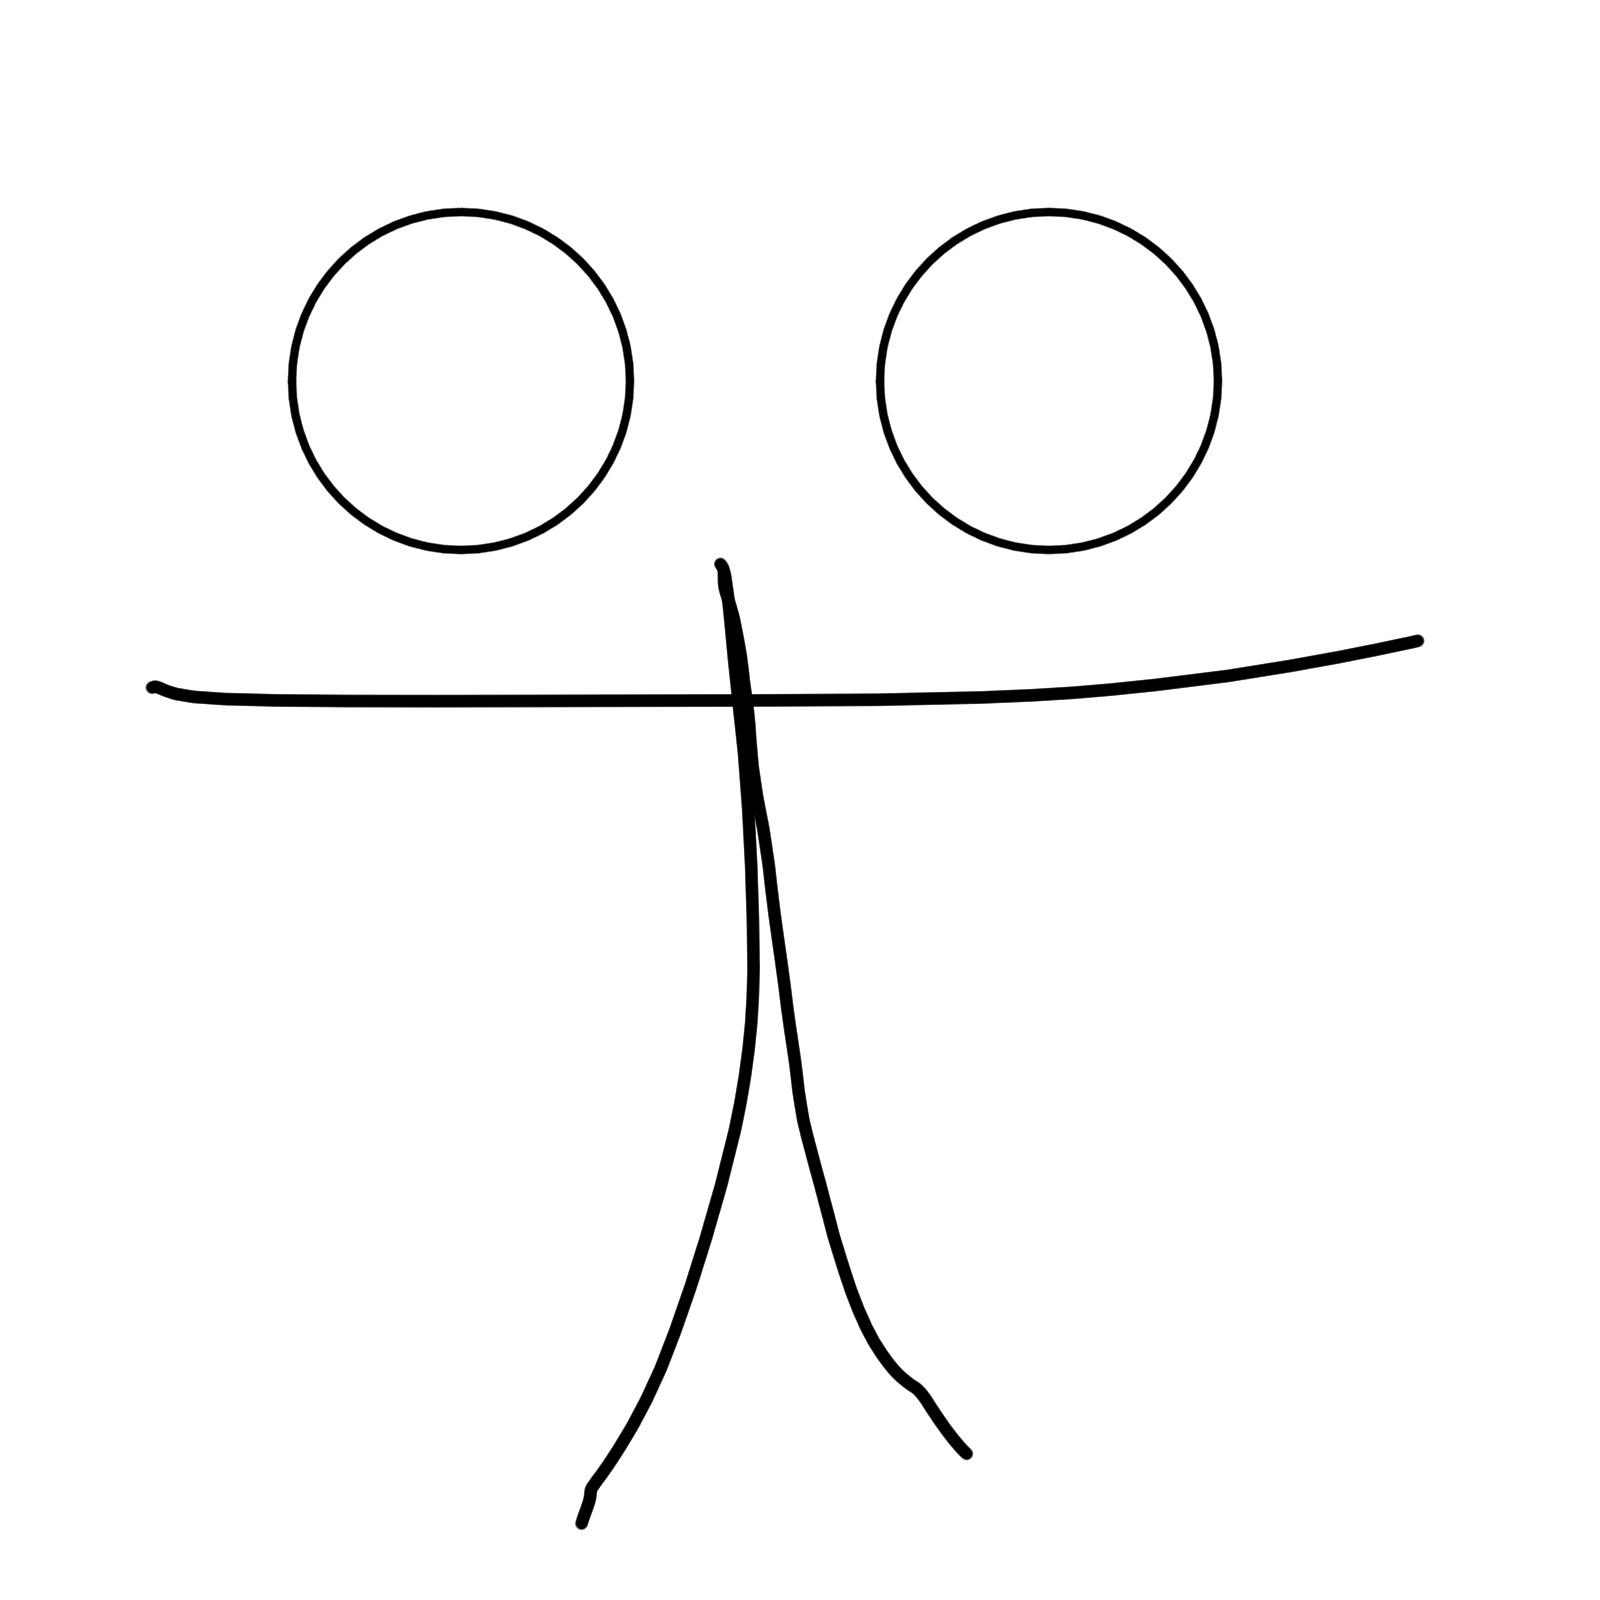
\includegraphics[width=\linewidth, height=20mm]{img/05keyframe}
    \end{minipage} 
    & 
    \begin{minipage}{.15\textwidth}
      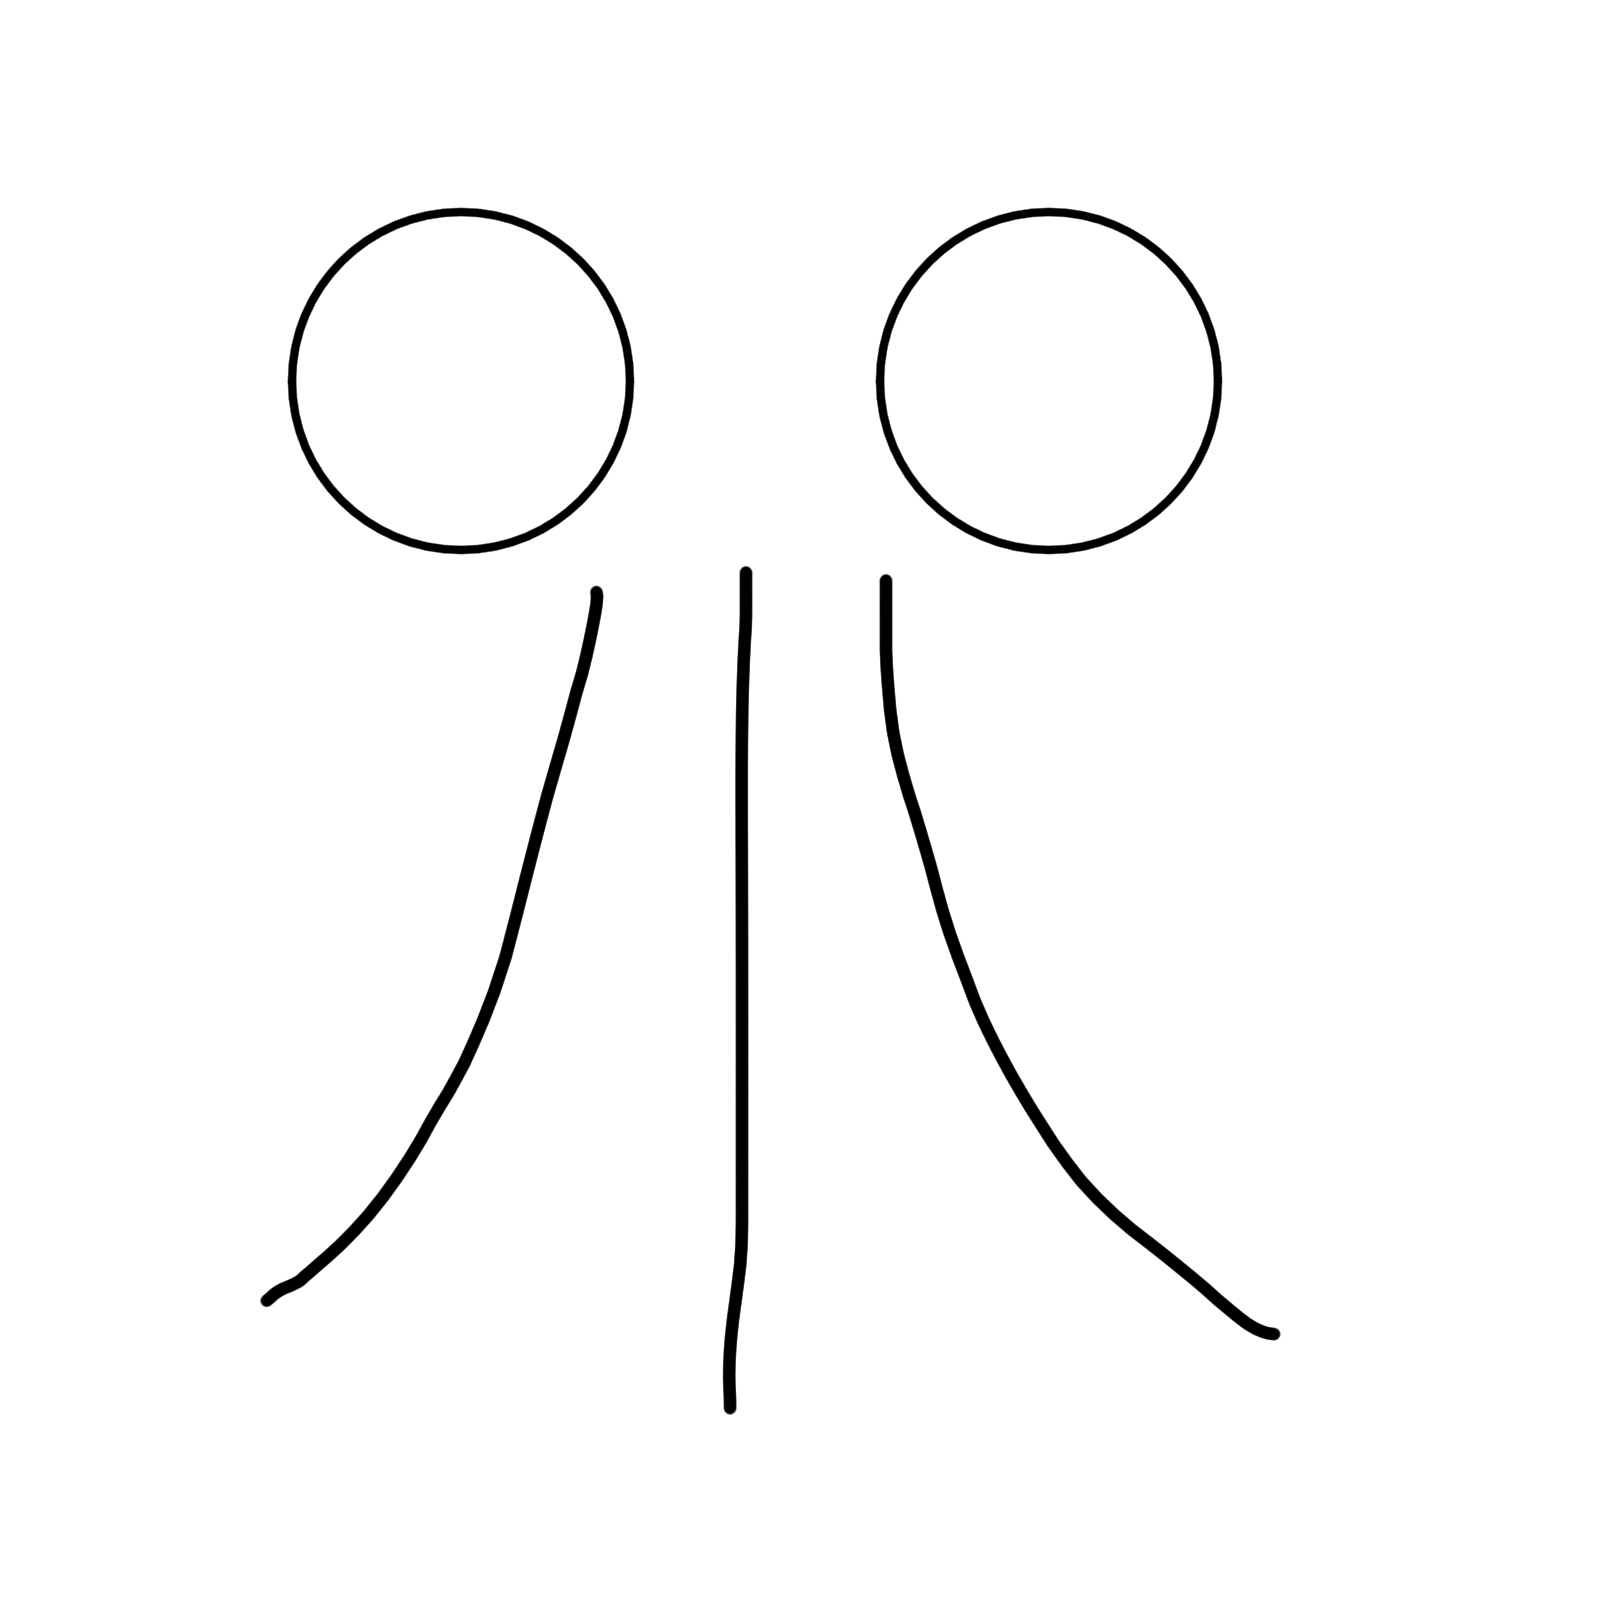
\includegraphics[width=\linewidth, height=20mm]{img/06keyframe}
    \end{minipage} 
    \\ \hline
    4 LOA 
    &
    \begin{minipage}{.15\textwidth}
      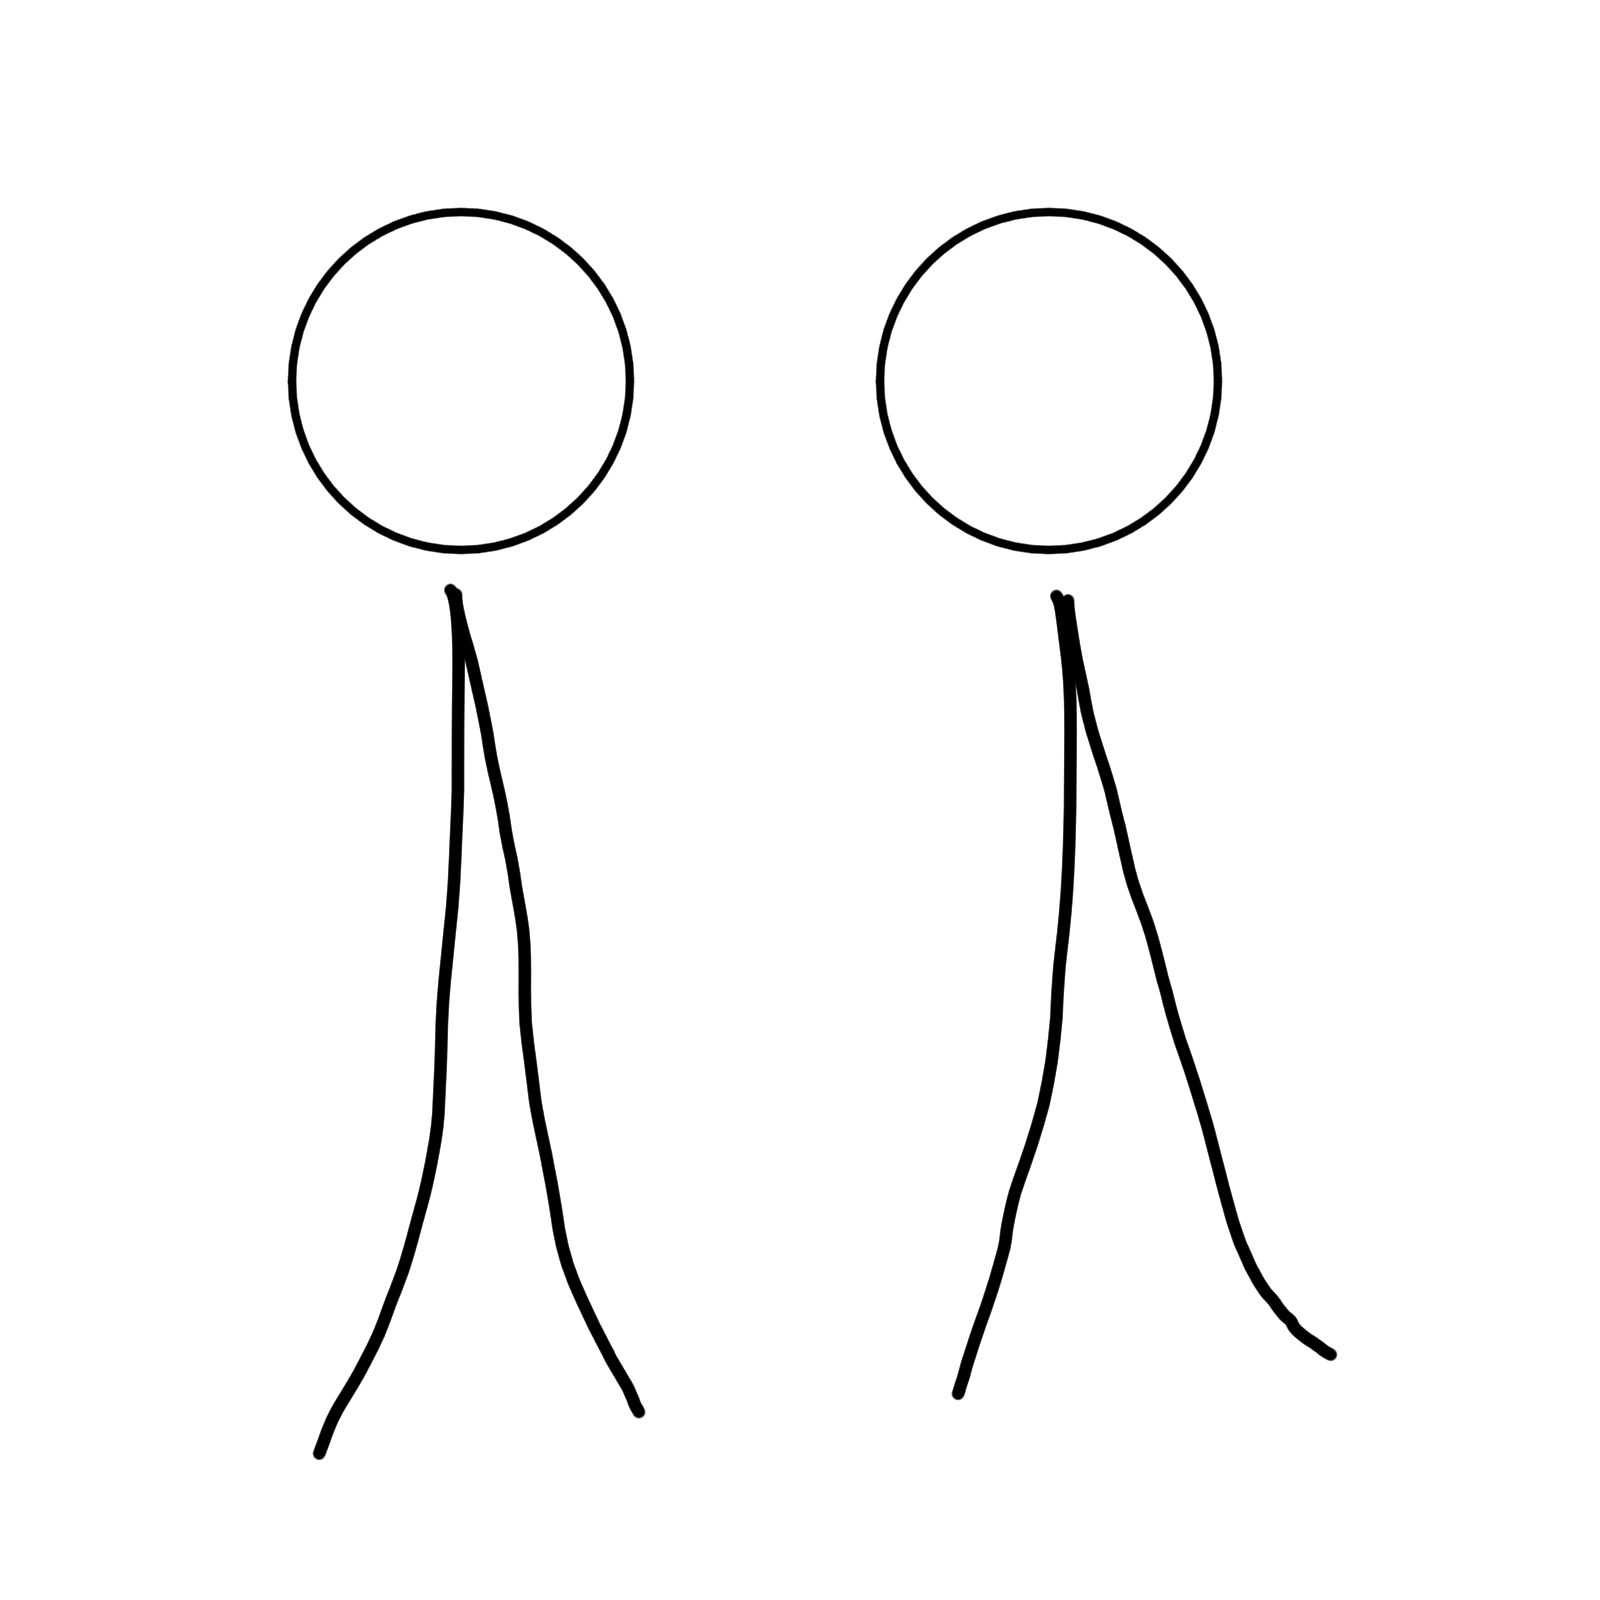
\includegraphics[width=\linewidth, height=20mm]{img/4loa_separate_keyframe}
    \end{minipage}
    &
    \begin{minipage}{.15\textwidth}
      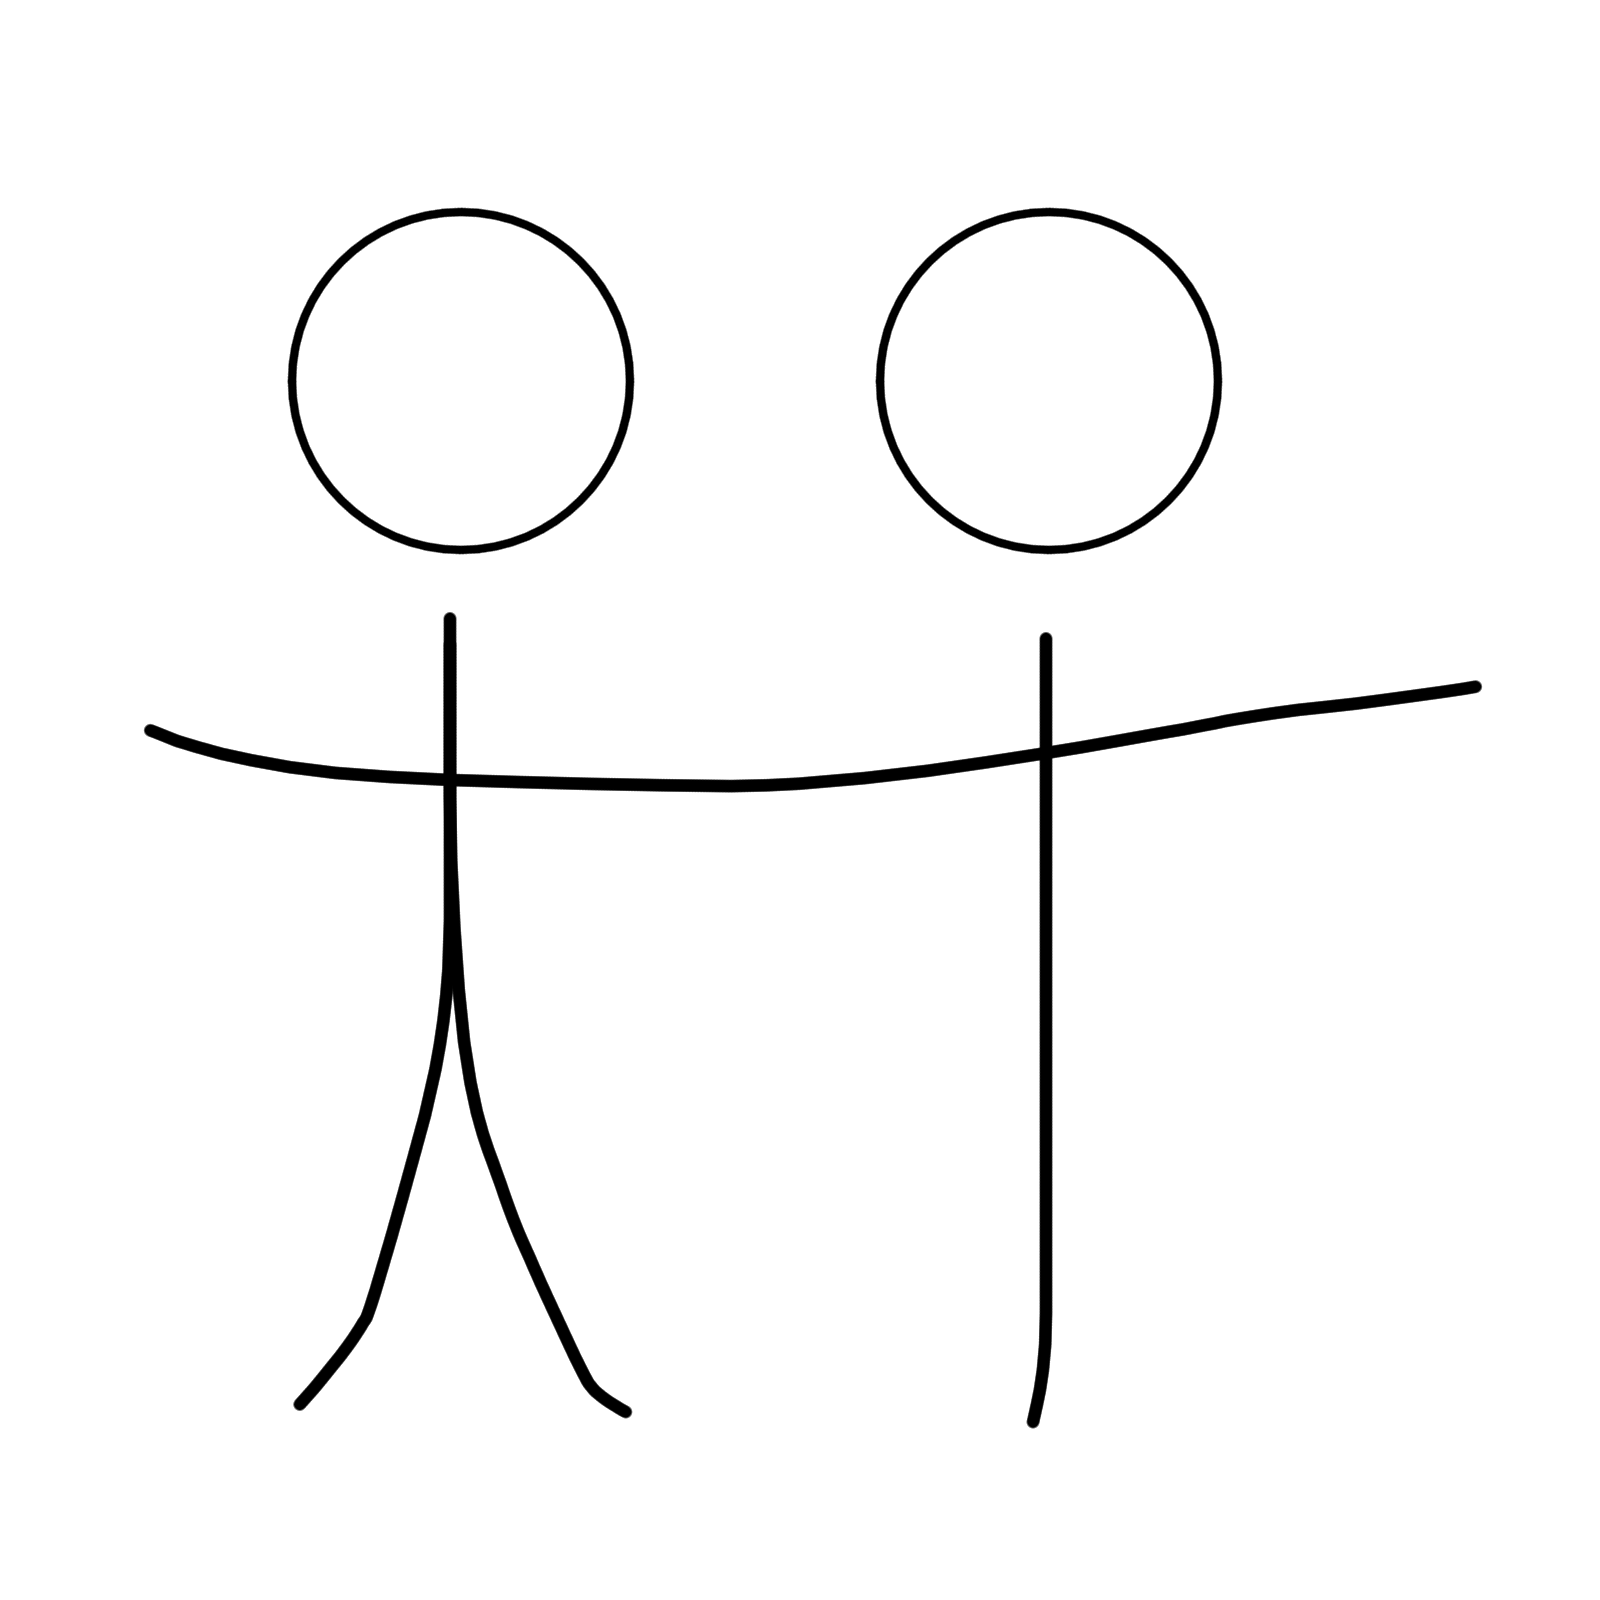
\includegraphics[width=\linewidth, height=20mm]{img/07keyframe}
    \end{minipage}
    &
    \begin{minipage}{.15\textwidth}
      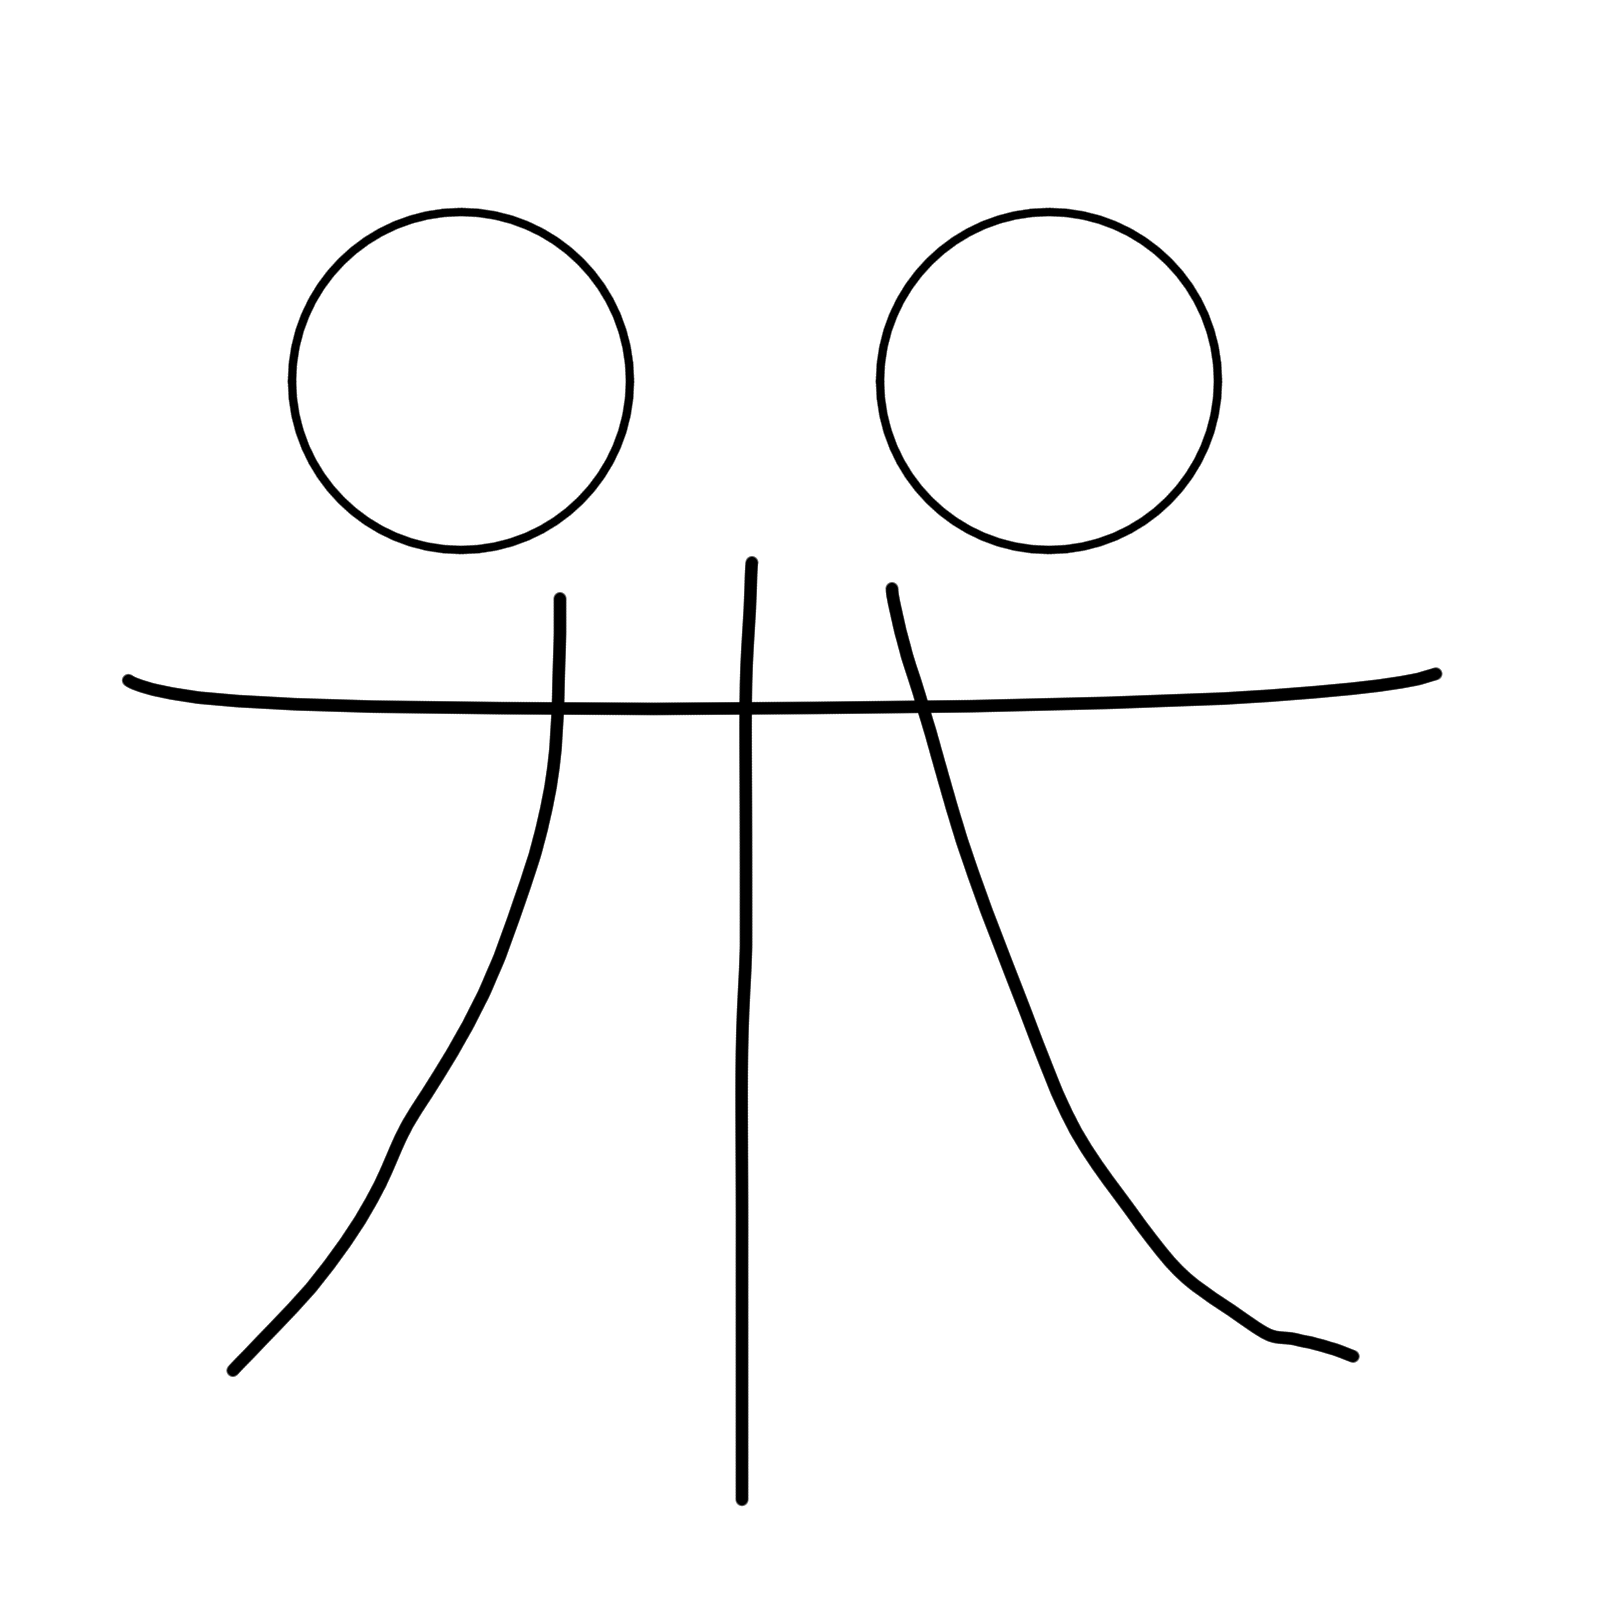
\includegraphics[width=\linewidth, height=20mm]{img/08keyframe}
    \end{minipage} 
    & 
    \begin{minipage}{.15\textwidth}
      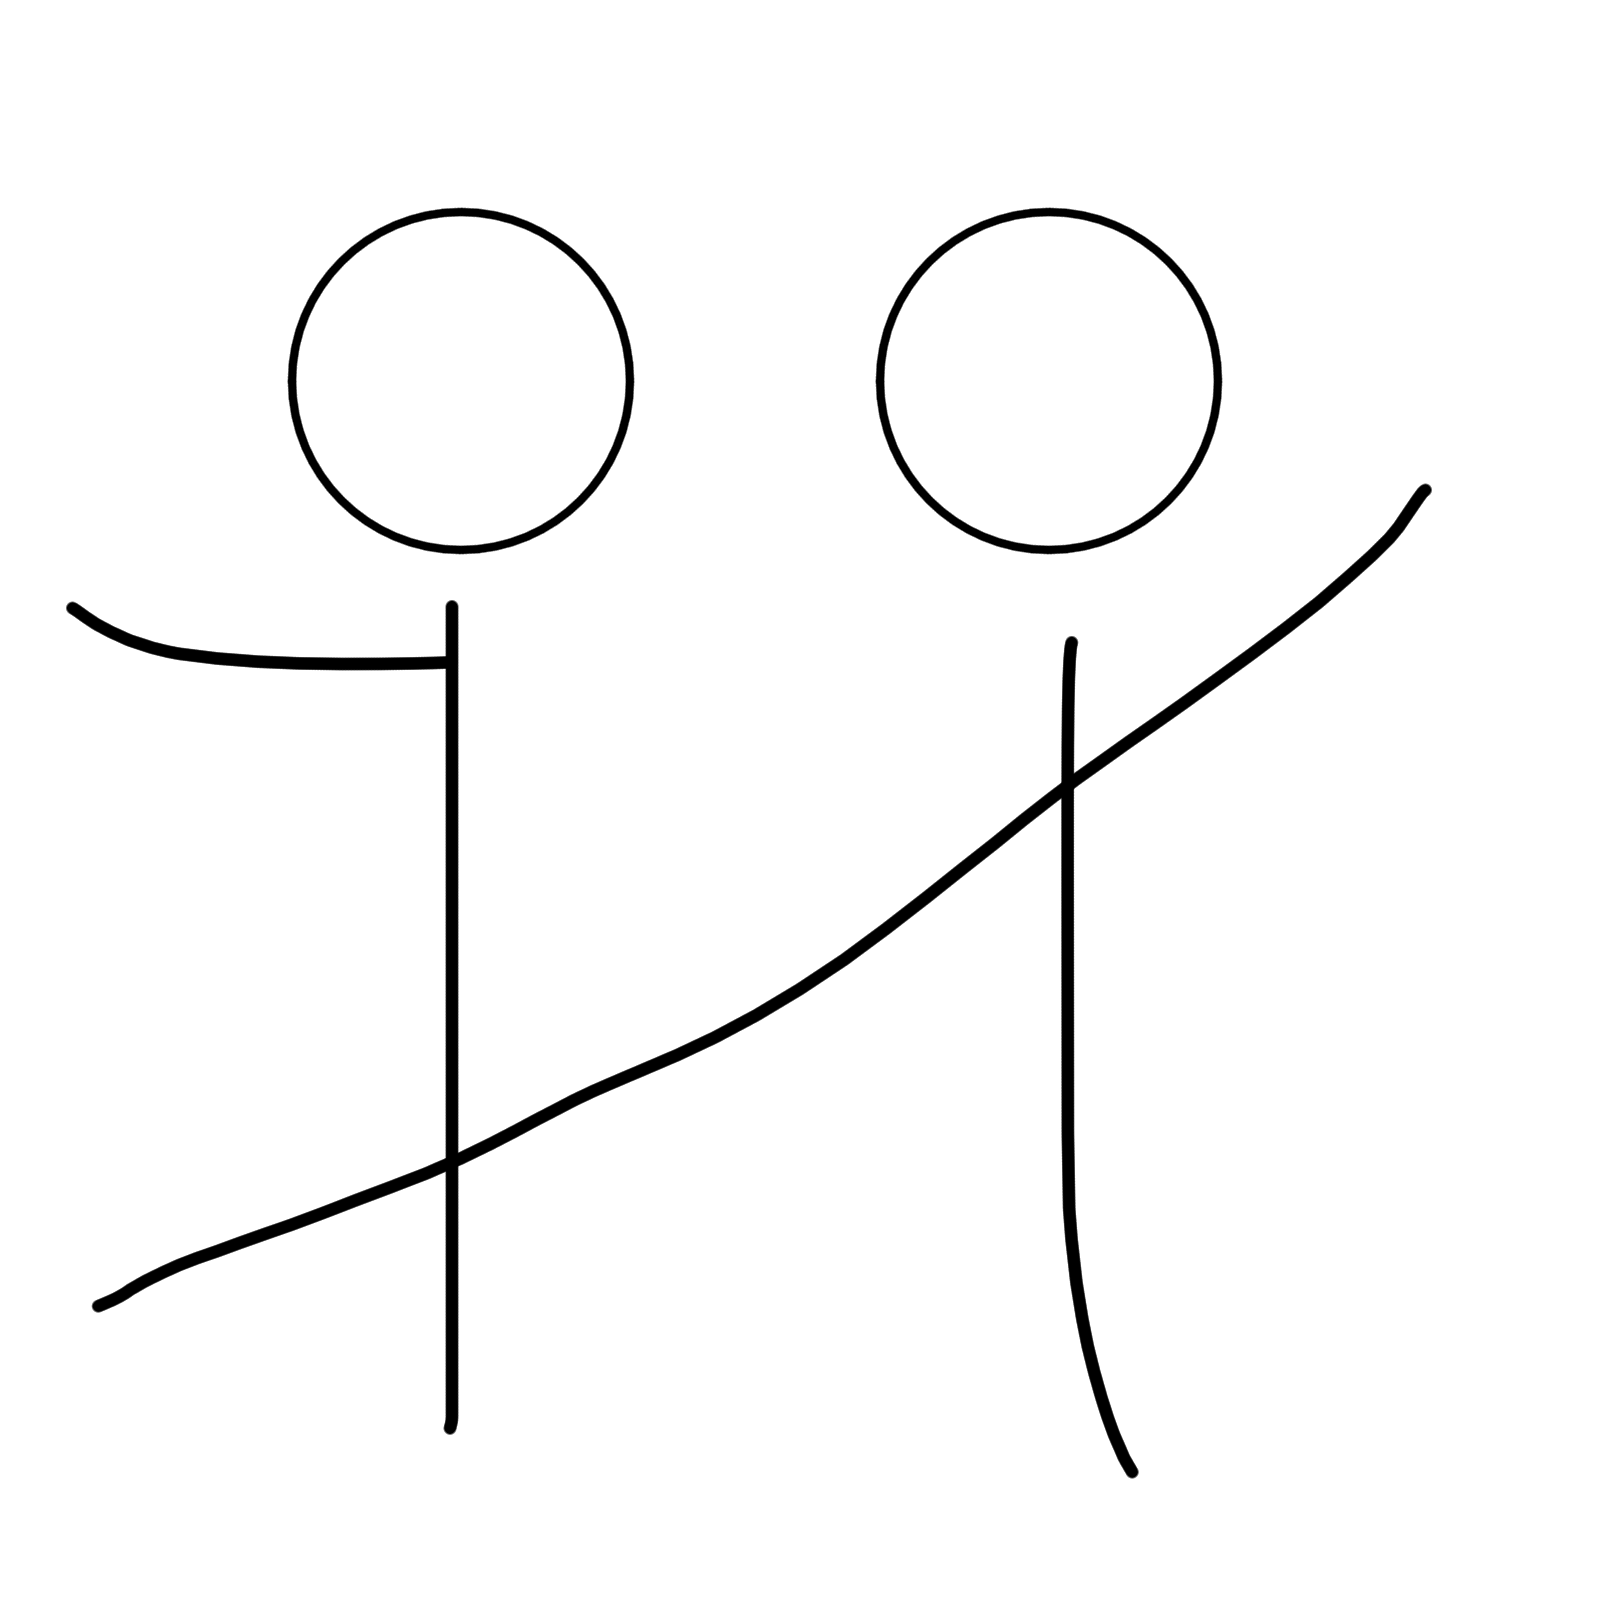
\includegraphics[width=\linewidth, height=20mm]{img/09keyframe}
    \end{minipage} 
    \\ \hline 
    &
    \begin{minipage}{.15\textwidth}
      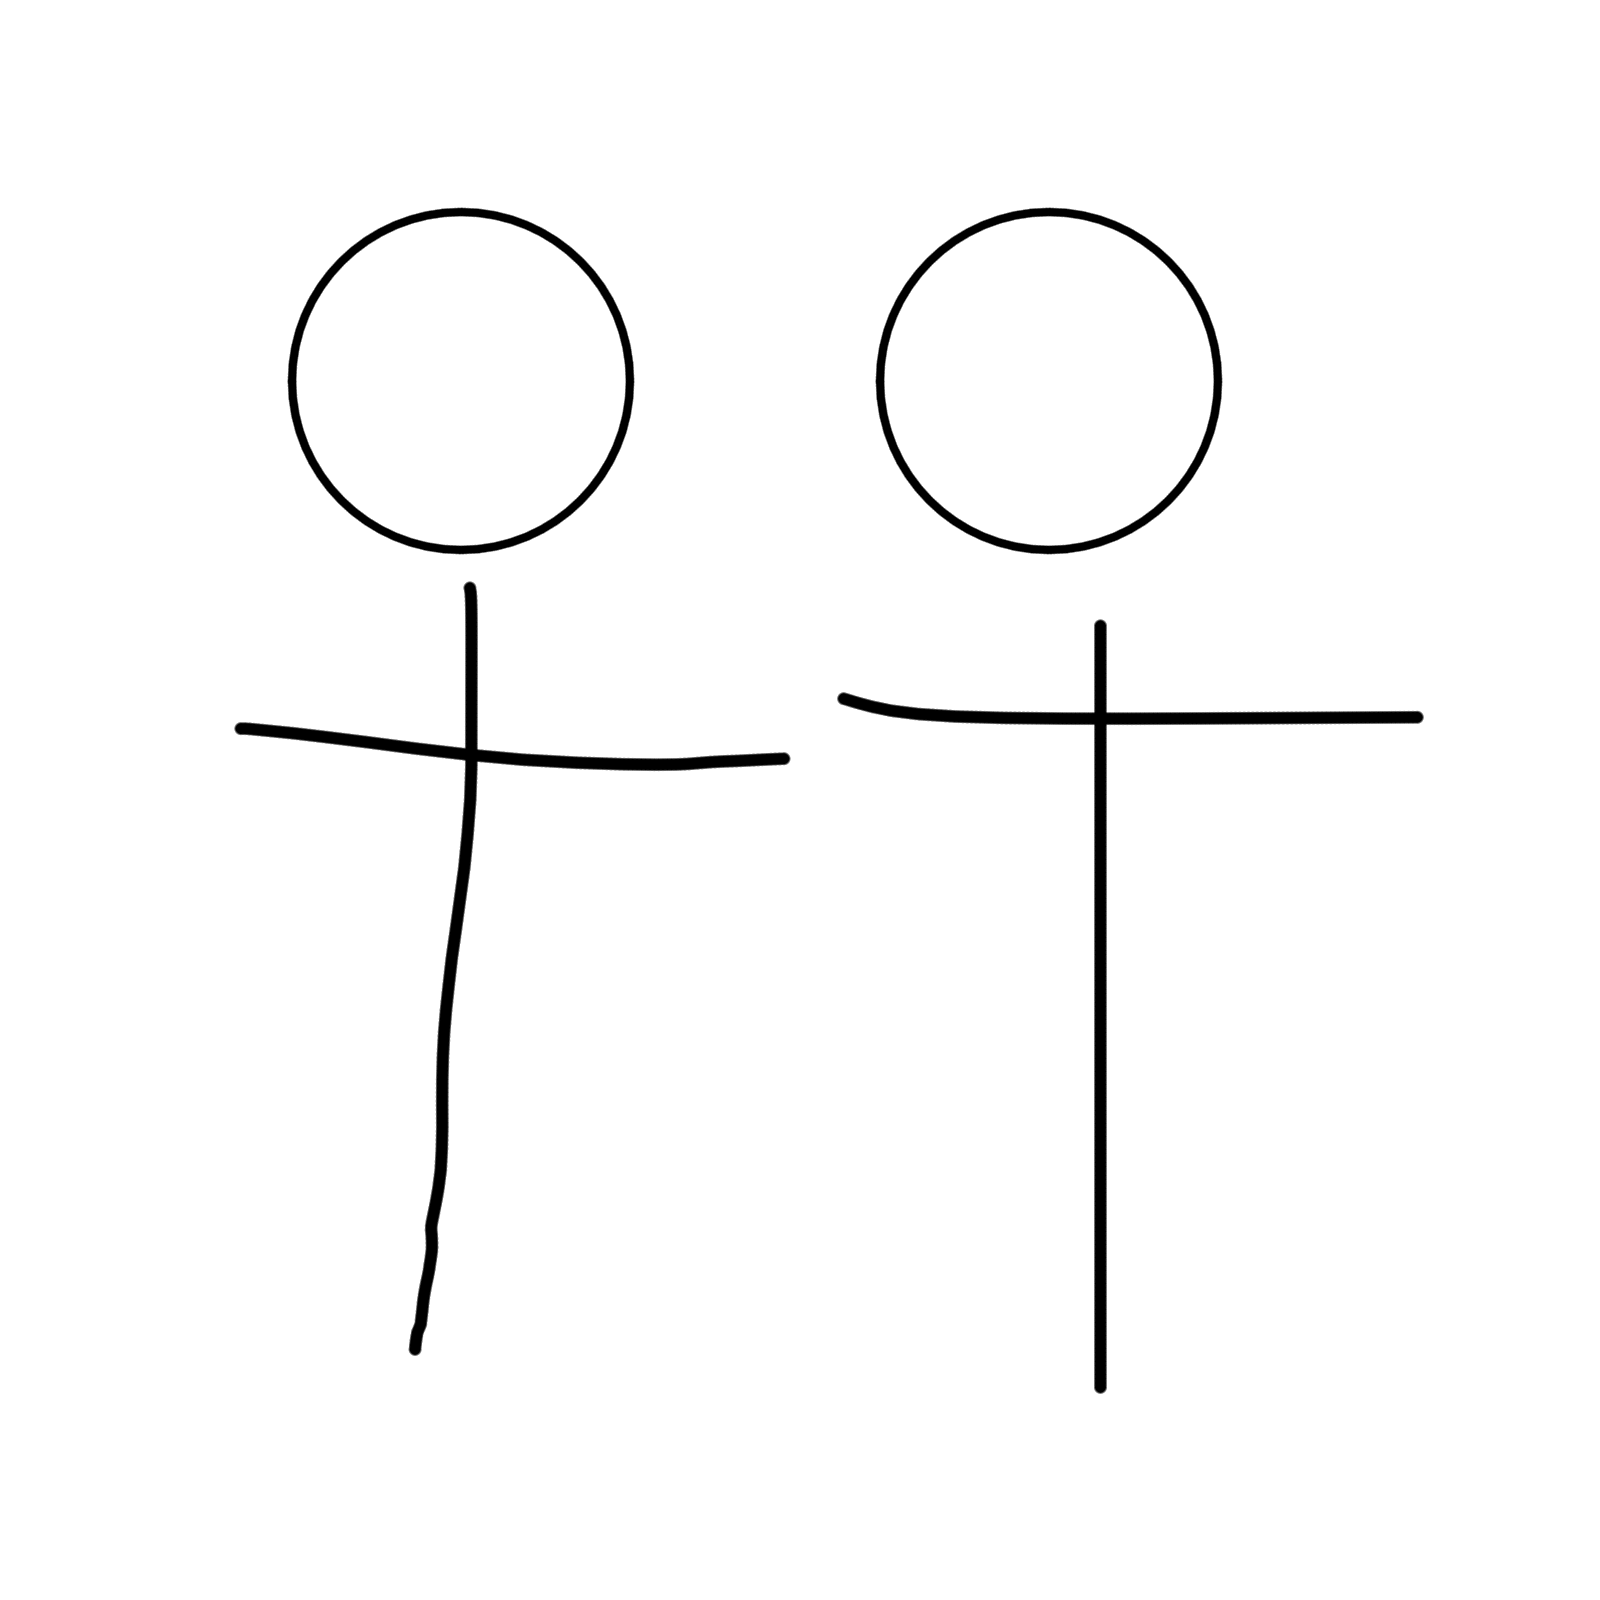
\includegraphics[width=\linewidth, height=20mm]{img/4-1loa_separate_keyframe}
    \end{minipage}
    & & & 
    \\ \hline
    5 LOA 
    &
    \begin{minipage}{.15\textwidth}
      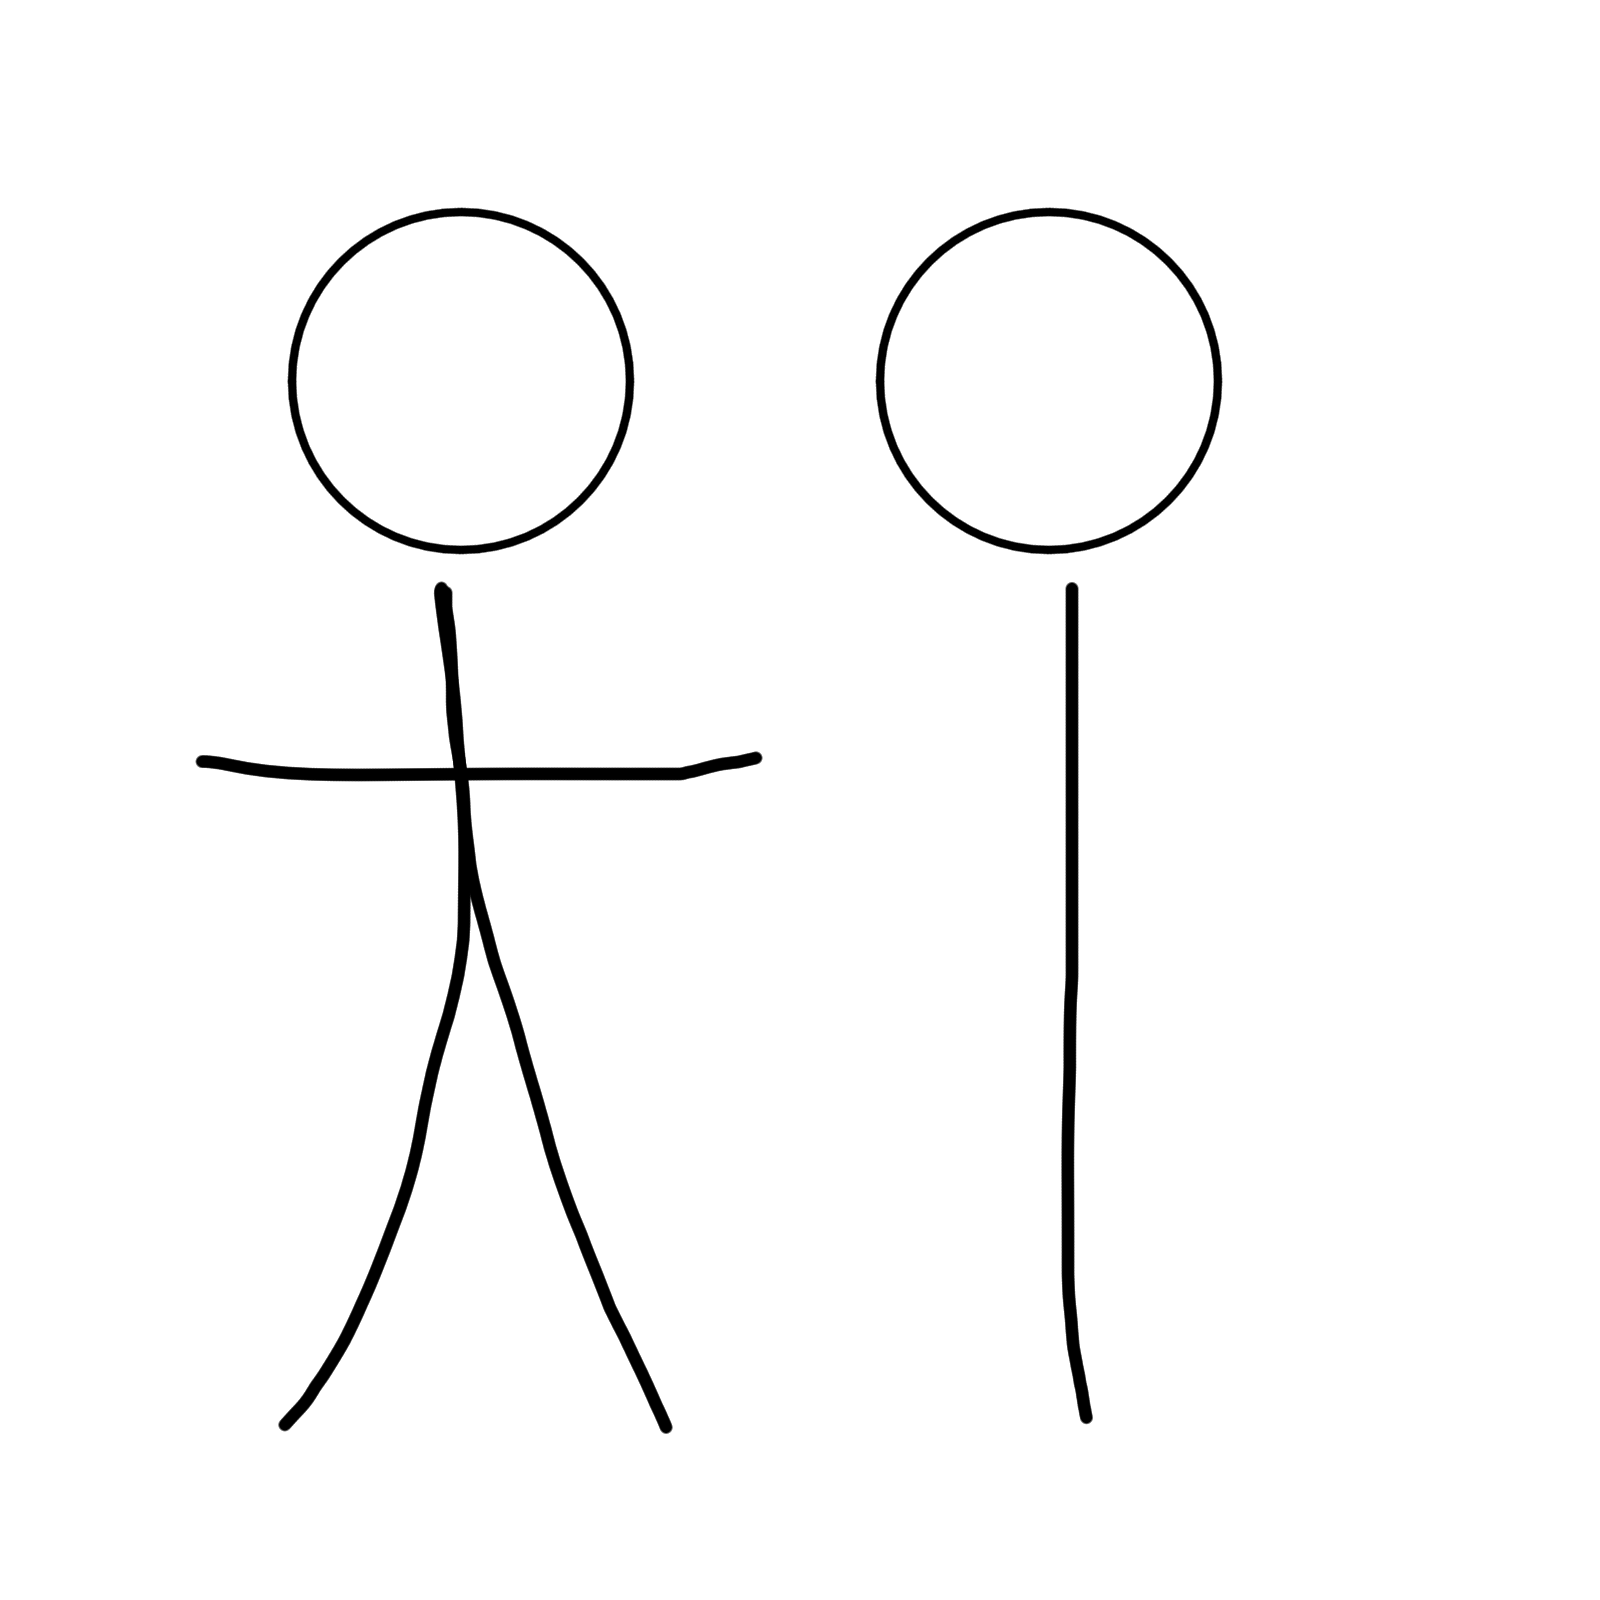
\includegraphics[width=\linewidth, height=20mm]{img/5loa_separate_keyframe}
    \end{minipage}
    &
    \begin{minipage}{.15\textwidth}
      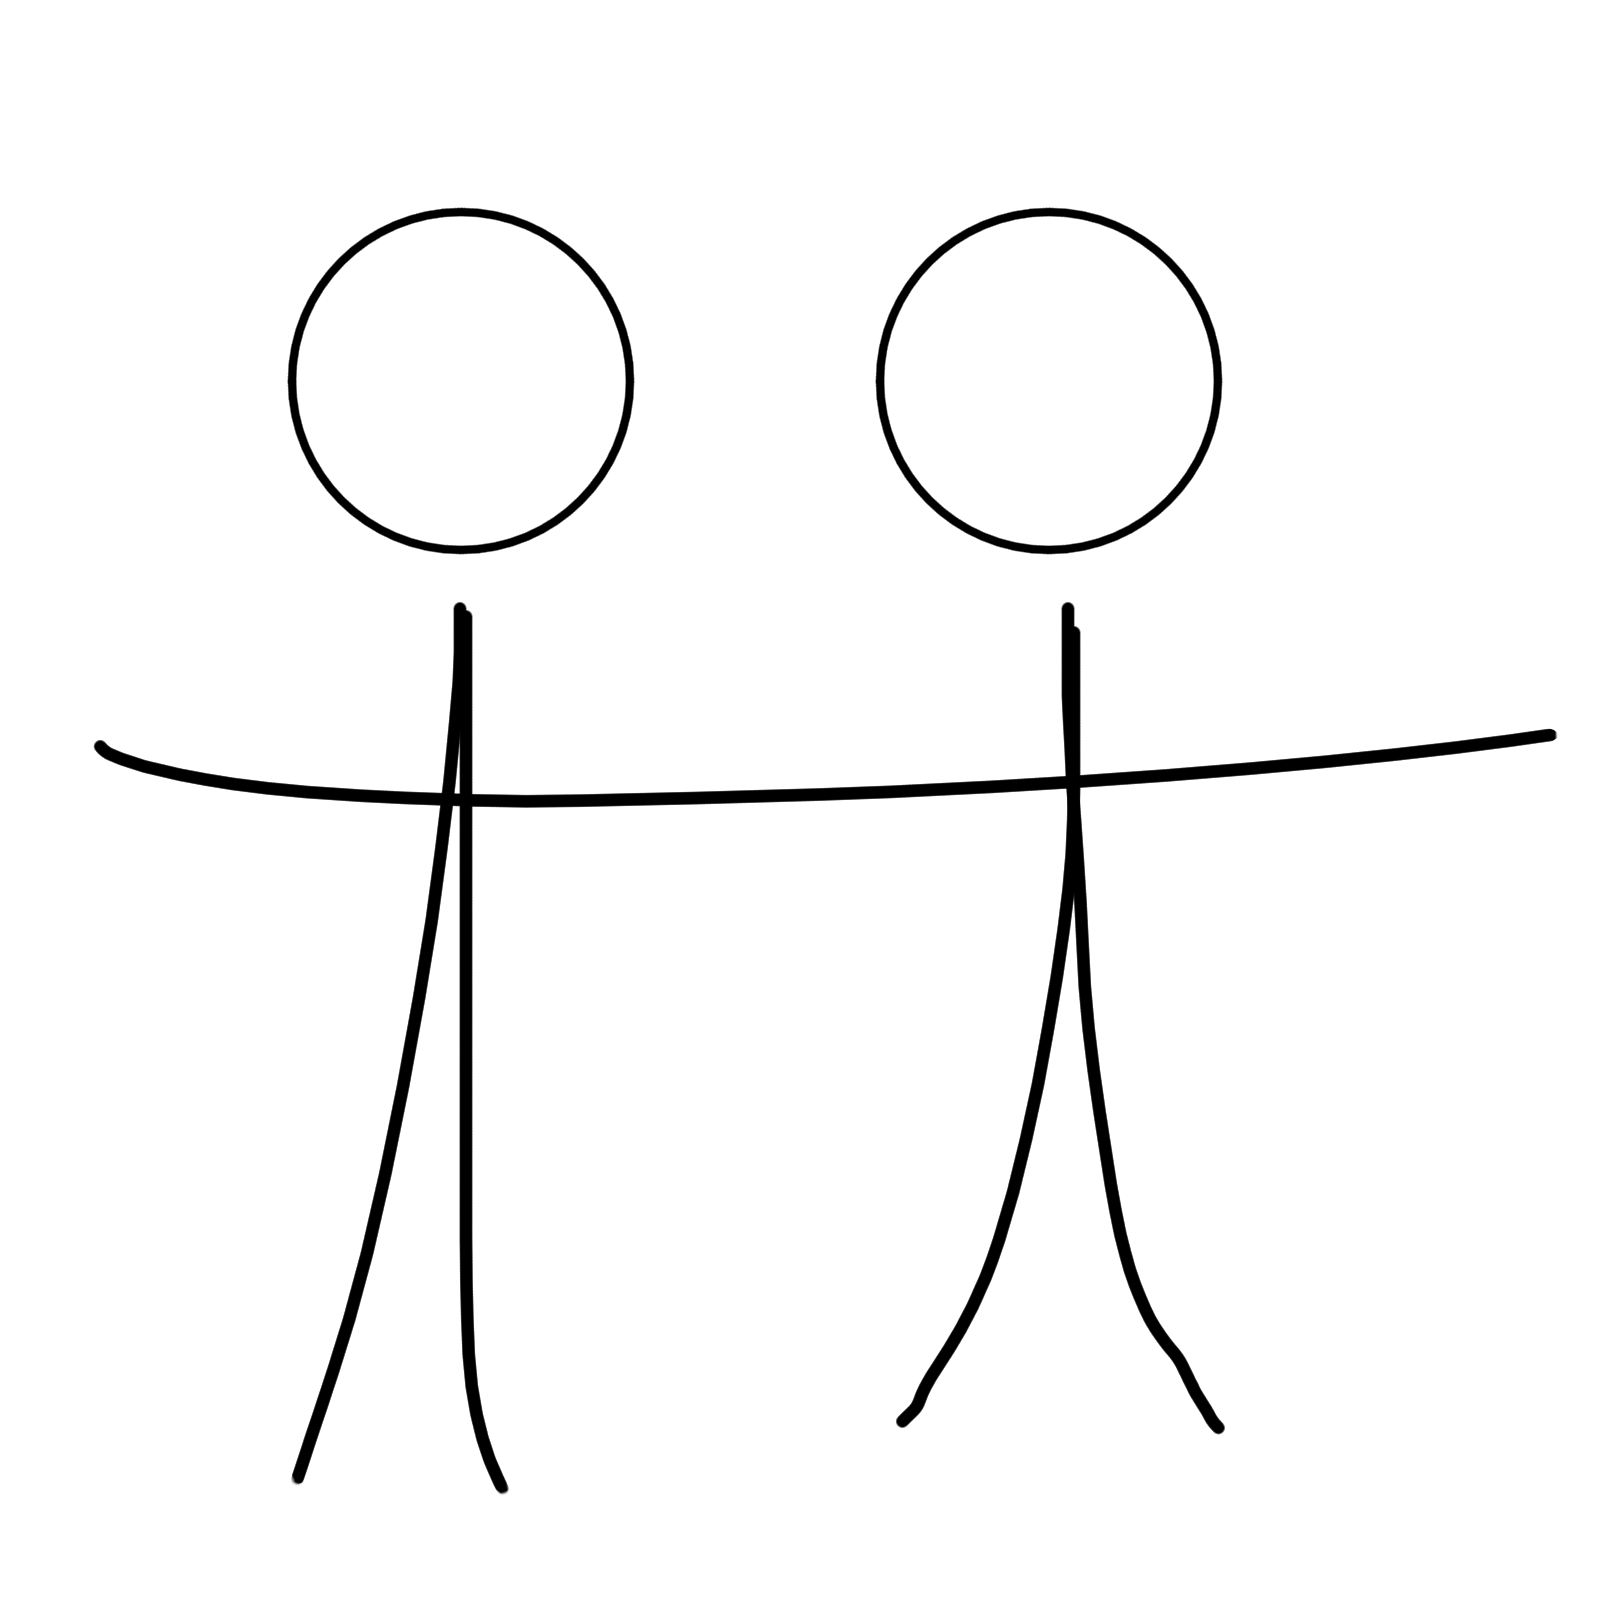
\includegraphics[width=\linewidth, height=20mm]{img/10keyframe}
    \end{minipage} & & 
    \\ \hline
    6 LOA 
    &
    \begin{minipage}{.15\textwidth}
      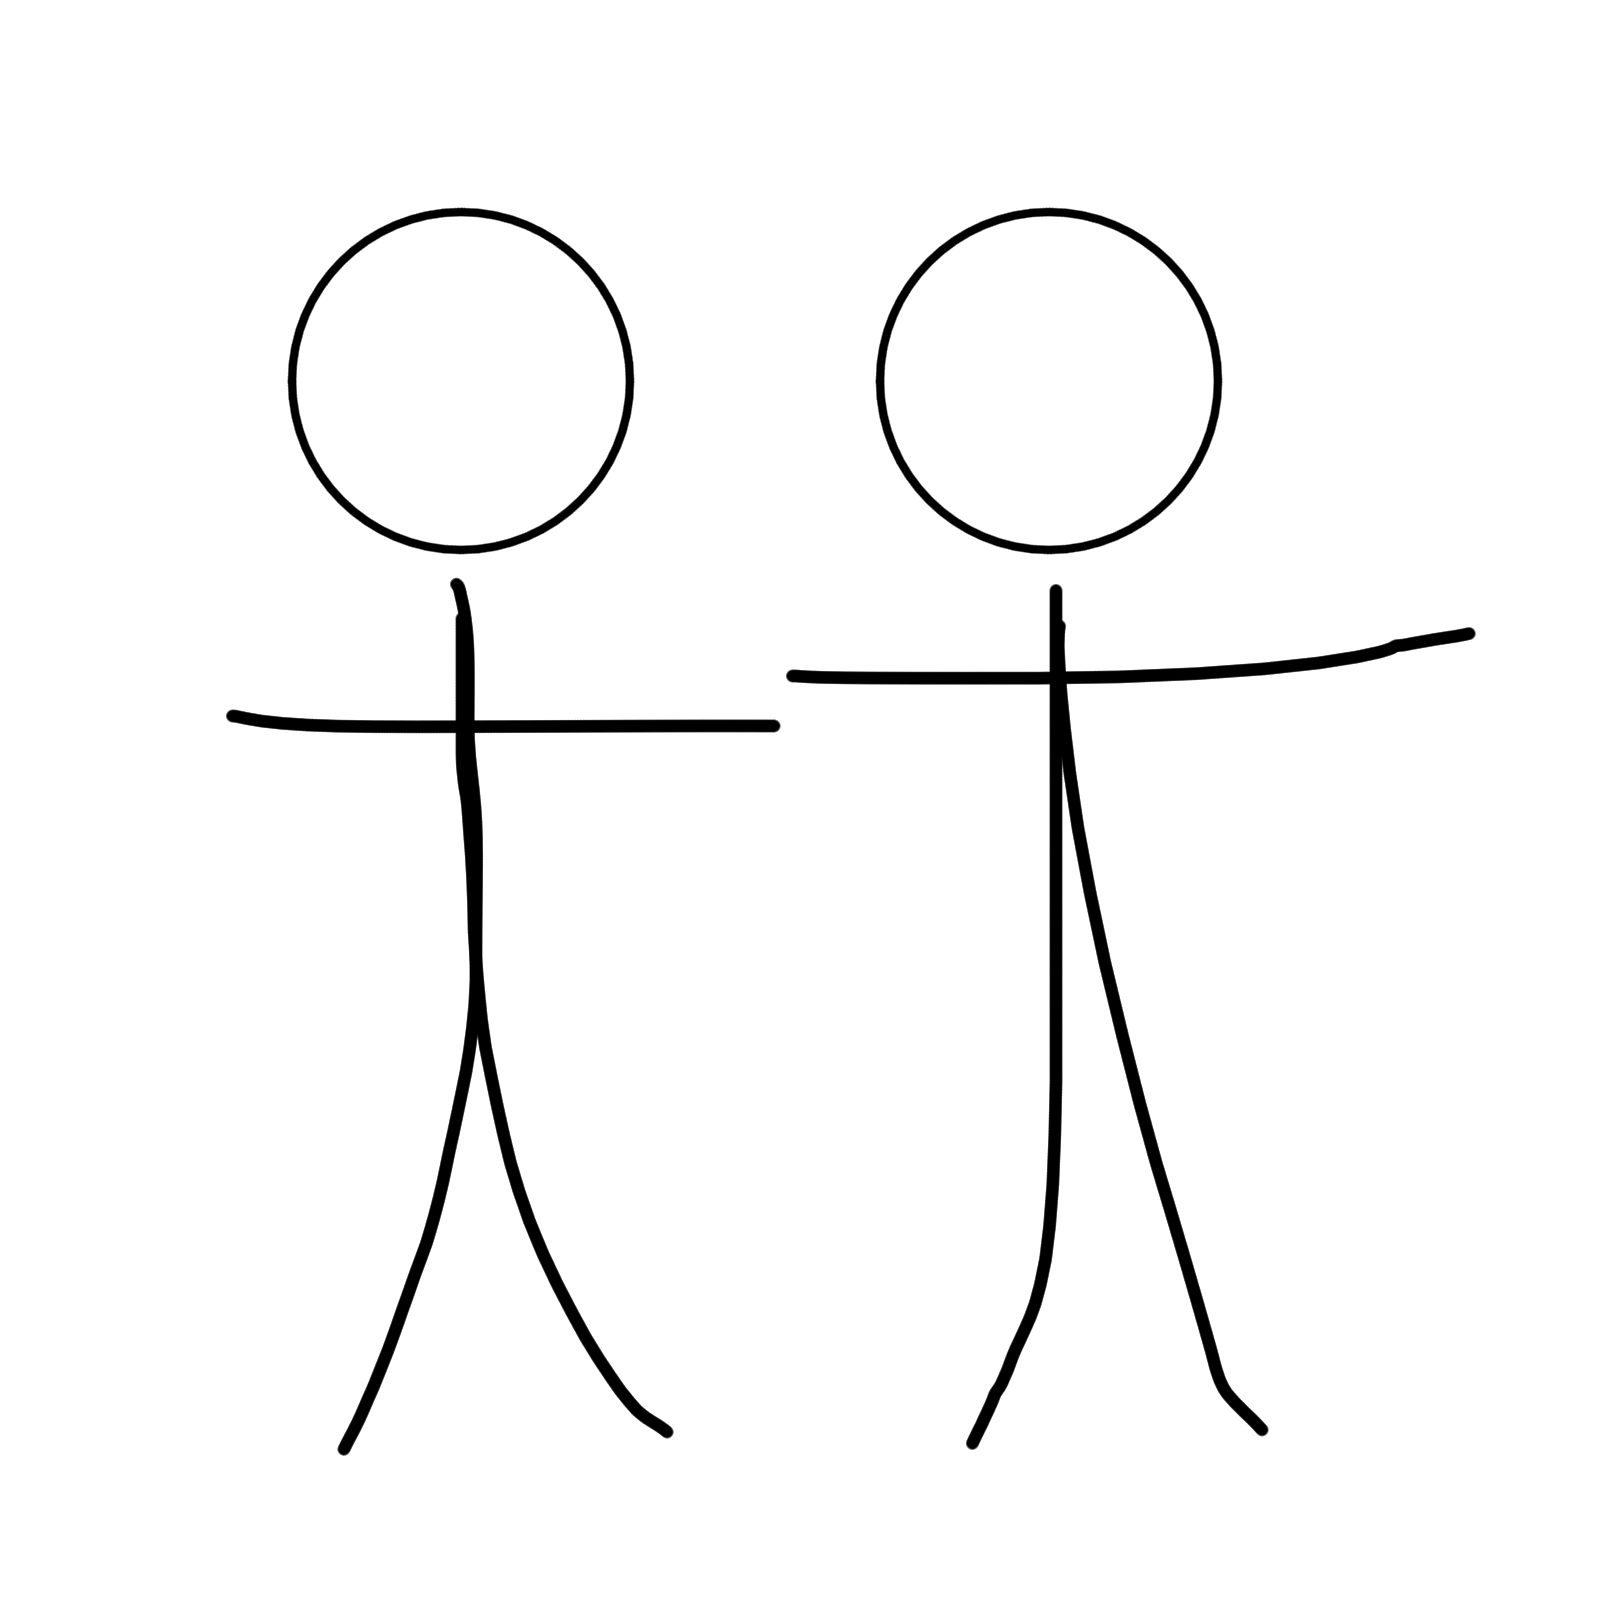
\includegraphics[width=\linewidth, height=20mm]{img/6loa_separate_keyframe}
    \end{minipage}
    & & & 
    \\ \hline
  \end{tabular}
  \caption{Types of Keyframes for Two Dancing Characters}
  \label{LOAChart}
\end{table}

\newpage
There are 6 poses combinations for the characters separately. The asymmetrical poses for the odd number of LOAs can be mirrored (for 3 and 5 LOAs); therefore there are actually 8 poses for two characters separately. There are 10 combinations for the characters together, treated as one character. There are 2 poses which can be mirrored, so there are actually 12 poses together. Overall, 20 poses exist for 2 articulated humanoid characters.

\backmatter

\bibliographystyle{plain} 
\nocite{*}
\bibliography{bibfile}


\end{document}